% !TeX program = pdflatex
% ============================================================
% OPERATING-VALUE SENSITIVITY — RESEARCH PAPER TEMPLATE
% Condensed scientific-paper format for a thesis-based valuation
% Target: <= 10 pages INCLUDING references.
% ============================================================

\documentclass[9pt,a4paper]{extarticle}

% ---------- Language & typography ----------
\usepackage[T1]{fontenc}
\usepackage[utf8]{inputenc}
\usepackage[english]{babel}
\usepackage{newtxtext,newtxmath}
\linespread{0.98}
\usepackage[protrusion=true,expansion=true]{microtype}
\usepackage[
  top=1.65cm,
  bottom=1.85cm,
  left=1.55cm,
  right=1.55cm,
  headheight=16pt,
  headsep=10pt,
  footskip=18pt
]{geometry}

% ---------- Core packages ----------
\usepackage{graphicx}
\usepackage{pdfpages}
\usepackage{xcolor}
\usepackage{booktabs}
\usepackage{array}
\usepackage{tabularx}
\usepackage{siunitx}
\usepackage{amsmath,mathtools,bm}
\usepackage{enumitem}
\usepackage{multicol}
\usepackage{caption}
\usepackage{subcaption}
\usepackage{float}
\usepackage{fancyhdr}
\usepackage{titlesec}
\usepackage[most]{tcolorbox}
\usepackage{natbib}
\usepackage{hyperref}
\usepackage[nameinlink,noabbrev]{cleveref}

% ---------- Palette ----------
% Academic first; club identity is intentionally subtle.
\definecolor{ink}{RGB}{29,29,31}
\definecolor{muted}{RGB}{92,92,98}
\definecolor{rulegray}{RGB}{180,180,184}
\definecolor{papergray}{RGB}{241,241,242}
\definecolor{brand}{RGB}{80,26,176}
\definecolor{accent}{RGB}{180,162,47}

% ---------- Metadata: edit these only ----------
\newcommand{\PaperType}{RESEARCH ARTICLE}
\newcommand{\PaperTitle}{Operating-Value Sensitivity for Barrick Mining}
\newcommand{\ShortTitle}{OPERATING-VALUE SENSITIVITY — BARRICK MINING CORPORATION}
\newcommand{\PaperSubtitle}{A controlled comparison of option-implied gold-price laws}
\newcommand{\PreparedDate}{07/09/2026}
\newcommand{\RevisedDate}{07/09/2026}
\newcommand{\PaperID}{Working Paper}
\newcommand{\JELCodes}{G12; G13; G31; C32; C53; C61; C63}

% Research teams. Keep team ownership visible rather than flattening the
% project into a single long author line.
\newcommand{\TeamOne}{Stefano Falcione; Marco Fracca}
\newcommand{\TeamTwo}{Filippo Triassi; Giorgio Zoccatelli}
\newcommand{\TeamThree}{Andrea Rostagno; Francesco Florio}
\newcommand{\TeamFour}{Giacomo Scali; Jacopo Foralosso}
\newcommand{\TeamFive}{Federico Vesco; Lorenzo Pietra; Bader Moussaif}
\newcommand{\TeamSix}{Davide Sisto; Matteo Armando}
\newcommand{\TeamSeven}{Davide D'Amico; Pietro Weisz}
\newcommand{\TeamEight}{Salvatore Gabriele Messina; Alessandro Coco}

% Abstract intentionally excludes numerical results. Detailed calibration,
% model-comparison statistics and valuation percentiles belong in Results.
\newcommand{\PaperAbstract}{%
This study audits the sensitivity of an unreconciled Barrick operating-value proxy to alternative option-implied gold-price laws. Eight student teams connect probability, econometrics, simulation, operating forecasts and a common discounted-margin mapping. Black--Scholes, Heston, Bates and Bates--Hawkes are fitted to the same 64 GLD calls dated 2 September 2026. A calibration audit retains feasible nested candidates and improves the previously reported Bates and Hawkes fits; historical out-of-sample scores remain a separate, frozen experiment. Production, unit costs and annual discount-rate shocks are shared across 8,192 simulated paths. The reported quantities are aggregate operating proxies under explicit terminal conventions: no net-debt, ownership or diluted-share bridge is asserted. Option-implied risk-neutral dynamics combined with an assumed WACC do not constitute a validated corporate valuation or physical forecast. Signed perpetuity and five-year-only closures expose the sensitivity to terminal assumptions. Numerical checks also show that small cross-model differences in medians are not stable evidence of economic ranking. The contribution is a reproducible, controlled research experiment with explicit limits on accounting, probability measure, option conventions, extrapolation and statistical inference. Results are neither fair values nor price targets, investment recommendations or evidence of market mispricing.%
}

% ---------- Hyperlinks ----------
\hypersetup{
  colorlinks=true,
  linkcolor=brand,
  citecolor=brand,
  urlcolor=brand,
  pdftitle={\PaperTitle},
  pdfauthor={Starting Finance Club PoliTo Research}
}

% ---------- Global paragraph settings ----------
\setlength{\parindent}{1em}
\setlength{\parskip}{0pt}
\setlength{\columnsep}{0.62cm}
\setlength{\columnseprule}{0pt}
\raggedbottom

% ---------- Section style ----------
\titleformat{\section}
  {\normalfont\bfseries\fontsize{9.4}{10.8}\selectfont\color{ink}\raggedright\MakeUppercase}
  {\thesection}{0.65em}{}
\titlespacing*{\section}{0pt}{9pt}{3pt}

\titleformat{\subsection}
  {\normalfont\bfseries\fontsize{9.1}{10.5}\selectfont\color{ink}\raggedright}
  {\thesubsection}{0.55em}{}
\titlespacing*{\subsection}{0pt}{6pt}{2pt}

\titleformat{\subsubsection}
  {\normalfont\itshape\fontsize{8.9}{10.3}\selectfont\color{ink}\raggedright}
  {\thesubsubsection}{0.5em}{}
\titlespacing*{\subsubsection}{0pt}{5pt}{1.5pt}

% ---------- Header / footer ----------
\pagestyle{fancy}
\fancyhf{}
\fancyhead[L]{\fontsize{7.3}{8.5}\selectfont\color{muted}\ShortTitle}
\fancyhead[R]{\fontsize{7.3}{8.5}\selectfont\color{muted}STARTING FINANCE CLUB POLITO — RESEARCH}
\fancyfoot[C]{\fontsize{7.1}{8}\selectfont\color{muted}\thepage}
\renewcommand{\headrulewidth}{0.35pt}
\renewcommand{\footrulewidth}{0pt}

\fancypagestyle{firstpage}{%
  \fancyhf{}
  \fancyfoot[C]{\fontsize{7.1}{8}\selectfont\color{muted}\thepage}
  \renewcommand{\headrulewidth}{0pt}
  \renewcommand{\footrulewidth}{0pt}
}

% ---------- Captions ----------
\captionsetup{
  hypcap=false,
  font=footnotesize,
  labelfont=bf,
  labelsep=period,
  justification=raggedright,
  singlelinecheck=false,
  skip=2pt
}

% ---------- Lists ----------
\setlist[itemize]{leftmargin=1.2em,itemsep=1pt,topsep=3pt,parsep=0pt}
\setlist[enumerate]{leftmargin=1.3em,itemsep=1pt,topsep=3pt,parsep=0pt}

% ---------- Tables ----------
\sisetup{
  detect-all,
  group-separator={,},
  group-minimum-digits=4,
  table-number-alignment=center
}
\renewcommand{\arraystretch}{1.08}

% ---------- Reusable scientific-paper boxes ----------
\newtcolorbox{findingbox}[1][Key finding]{
  colback=papergray,
  colframe=rulegray,
  boxrule=0.45pt,
  arc=0pt,
  left=5pt,right=5pt,top=4pt,bottom=4pt,
  before skip=5pt,after skip=5pt,
  fonttitle=\bfseries\fontsize{8.4}{9.5}\selectfont,
  title=#1
}

\newtcolorbox{methodbox}[1][Methodological note]{
  colback=brand!3,
  colframe=brand!35,
  boxrule=0.45pt,
  arc=0pt,
  left=5pt,right=5pt,top=4pt,bottom=4pt,
  before skip=5pt,after skip=5pt,
  fonttitle=\bfseries\fontsize{8.4}{9.5}\selectfont,
  title=#1
}

% ---------- Compact equation helper ----------
\newcommand{\E}{\mathbb{E}}
\newcommand{\Var}{\mathrm{Var}}
\newcommand{\Cov}{\mathrm{Cov}}
\newcommand{\Prob}{\mathbb{P}}
\newcommand{\dd}{\,\mathrm{d}}

% ---------- Title-page helpers ----------
\newcommand{\topmetadata}{%
  \begingroup
  \setlength{\parindent}{0pt}%
  \noindent
  \begin{minipage}[c]{0.75\textwidth}
    \fontsize{7.0}{8.4}\selectfont\color{muted}\PreparedDate
  \end{minipage}%
  \hfill
  \begin{minipage}[c]{0.19\textwidth}\raggedleft
    
\includegraphics[height=24pt]{img/Logo_SFClub_Polito.png}
  \end{minipage}\par
  \vspace{2pt}
  {\color{rulegray}\rule{\textwidth}{0.45pt}}\par
  \vspace{7pt}
  {\fontsize{7.5}{9}\selectfont\bfseries\textls[130]{\PaperType}\par}
  \vspace{12pt}
  \endgroup
}


% ---------- Research-team author grid ----------
\newcommand{\teamrow}[4]{%
  \textbf{Team #1}\enspace #2 & \textbf{Team #3}\enspace #4 \\
}

\newcommand{\authorgrid}{%
\begingroup
\setlength{\tabcolsep}{7pt}%
\renewcommand{\arraystretch}{1.23}%
\noindent\begin{tabularx}{\textwidth}{@{}>{\raggedright\arraybackslash}X>{\raggedright\arraybackslash}X@{}}
\teamrow{1}{\TeamOne}{2}{\TeamTwo}
\teamrow{3}{\TeamThree}{4}{\TeamFour}
\teamrow{5}{\TeamFive}{6}{\TeamSix}
\teamrow{7}{\TeamSeven}{8}{\TeamEight}
\end{tabularx}
\endgroup
}

% ---------- Abstract panel ----------
\newcommand{\abstractpanel}{%
\begin{tcolorbox}[
  colback=papergray,
  colframe=papergray,
  boxrule=0pt,
  arc=0pt,
  left=7pt,right=7pt,top=6pt,bottom=6pt,
  width=\linewidth
]
{\bfseries\fontsize{8.5}{10}\selectfont Abstract}\par\vspace{2pt}
{\fontsize{8.05}{9.75}\selectfont
\PaperAbstract\par}

\end{tcolorbox}
}

% ============================================================
% DOCUMENT
% ============================================================
\begin{document}
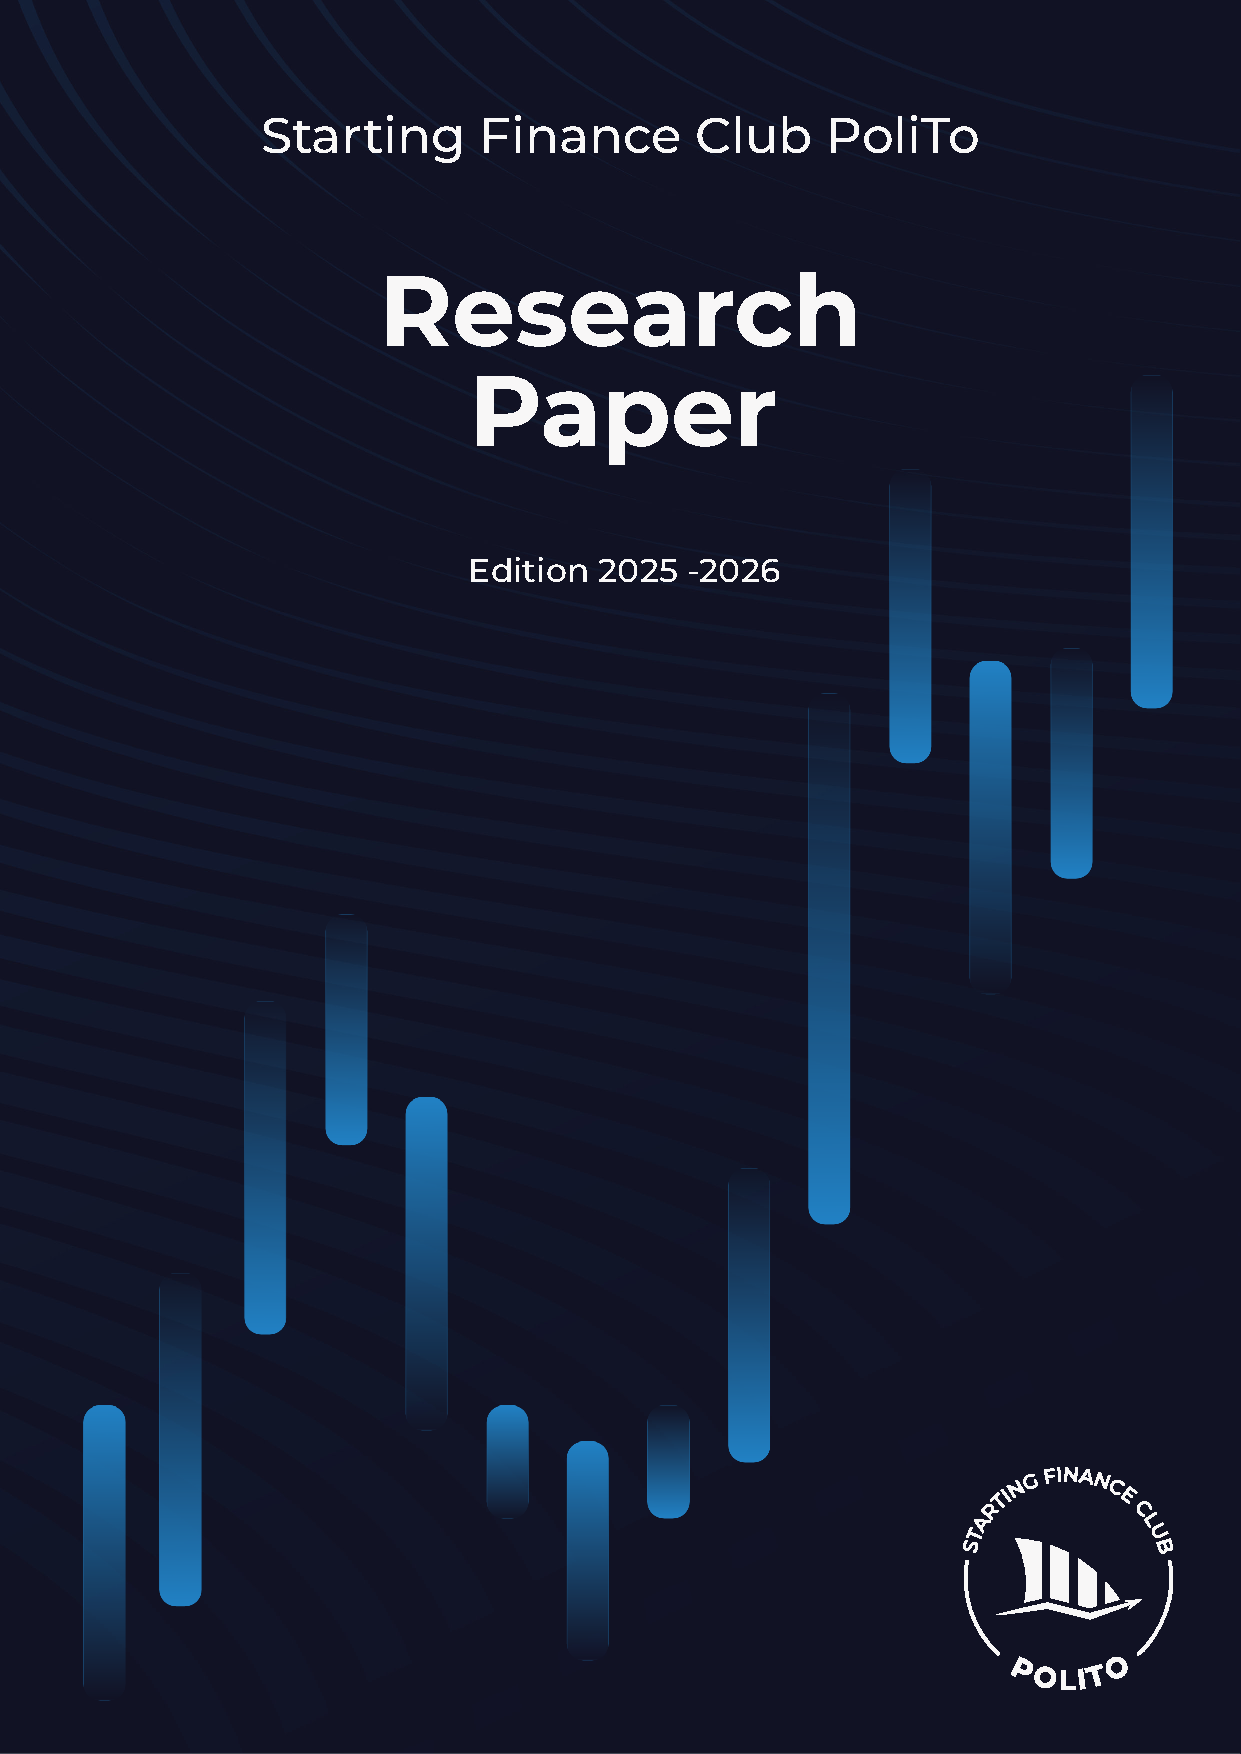
\includepdf[pages=1]{Copertina_research.pdf}
\setcounter{page}{1}
\thispagestyle{firstpage}
\fontsize{8.85}{10.55}\selectfont

% ----- Journal-like first-page masthead -----
\topmetadata

% ----- Title -----
{\noindent\fontsize{18.5}{21}\selectfont\bfseries\color{ink}\PaperTitle\par}
\vspace{3pt}
{\noindent\fontsize{9.3}{11}\selectfont\itshape\color{muted}\PaperSubtitle\par}
\vspace{11pt}

% ----- Authors: research teams paired across two columns -----
{\fontsize{7.85}{9.4}\selectfont\authorgrid}
\vspace{8pt}

% ----- Research affiliation + abstract layout inspired by academic journals -----
\noindent
\begin{minipage}[t]{0.28\textwidth}
  \vspace{0pt}
  {\fontsize{7.2}{8.85}\selectfont
  \textbf{Contacts --}\par
  \textbf{Starting Finance Club PoliTO}\par\vspace{3pt}
  \href{https://www.linkedin.com/company/startingfinance-club-polito}{\raisebox{-1pt}{
\includegraphics[height=8pt]{img/contact_linkedin.png}}\,LinkedIn}\enspace
  \href{https://sfclubpolito.it/}{\raisebox{-1pt}{
\includegraphics[height=8pt]{img/contact_website.png}}\,Website}\par
  \href{https://github.com/StartingFinanceClubPoliTo/Research}{\raisebox{-1pt}{
\includegraphics[height=8pt]{img/contact_github.png}}\,GitHub}\enspace
  \href{https://www.instagram.com/sfclubpolito}{\raisebox{-1pt}{
\includegraphics[height=8pt]{img/contact_instagram.png}}\,Instagram}\par
  \href{mailto:startingfinanceclub@studenti.polito.it}{\raisebox{-1pt}{
\includegraphics[height=8pt]{img/contact_email.png}}\,Institutional email}\par\vspace{3pt}
  \textbf{JEL classification}\par
  \JELCodes\par
  \vspace{3pt}
  \textbf{Discoveries}\par\vspace{2pt}
  Calibrated engines share one\par
  unreconciled operating contract.\par\vspace{3pt}
  {\setlength{\tabcolsep}{0pt}\renewcommand{\arraystretch}{1.18}%
  \begin{tabular}{@{}p{59pt}p{47pt}r@{}}
  Black--Scholes & \textcolor{brand!55}{\rule{40.00pt}{4pt}} & 60.10\\
  Heston & \textcolor{brand!65}{\rule{39.78pt}{4pt}} & 59.77\\
  Bates--Poisson & \textcolor{brand!75}{\rule{39.35pt}{4pt}} & 59.12\\
  Bates--Hawkes & \textcolor{brand}{\rule{39.82pt}{4pt}} & 59.82
  \end{tabular}}\par\vspace{3pt}
  Signed-terminal proxy; USD billion.\par
  Sensitivity only; not company value\par
  or a physical probability forecast.\par
  }
\end{minipage}%
\hfill
\begin{minipage}[t]{0.69\textwidth}
  \vspace{0pt}
  \abstractpanel
\end{minipage}

\vspace{9pt}

% ============================================================
% BODY — CONTINUOUS TWO-COLUMN FLOW
% Figures stay within the continuous two-column flow.
% ============================================================
\begin{multicols}{2}
\raggedcolumns
\section*{Research programme and collaboration}
This paper grew out of an eight-team project involving 17 students with complementary backgrounds in mathematics, data science, engineering, economics and finance. The size of the author group reflects a division of research responsibilities and a shared learning process: Teams 1--3 developed the mathematical, econometric and simulation foundations; Teams 4--5 built the operating and corporate-valuation layers; and Teams 6--8 studied gold-price dynamics, market evidence and option-implied calibration.

The extended \href{https://raw.githubusercontent.com/StartingFinanceClubPoliTo/Research/main/Barrick-Gold/Barrick\%20Mining\%20UNIFICATO/thesis/Articolo.pdf}{technical report} records definitions, derivations and implementation choices to establish a common technical language across these backgrounds. Teams worked on dedicated modules, then compared assumptions, revised their contributions and reconciled dates, units and interfaces before integration. The present paper condenses this work into a single auditable experiment. Together with the reproducible code, it demonstrates the group's existing research practice and provides a basis for developing a sustained student-led quantitative research team with academic guidance.

\section{Introduction}
A gold producer's value depends on the distribution of future commodity prices as well as its operating and financing assumptions. A single price path can hide this source of model risk. We ask how an unconstrained Barrick operating-proxy distribution changes when progressively richer gold-price processes are substituted within a common operating scenario and discounted-margin contract.

We compare Black--Scholes, Heston, Bates--Poisson and Full Bates--Hawkes calibrated to GLD options. Current-surface diagnostics and rolling out-of-sample tests distinguish fit from predictive performance; shared production, costs and WACC shocks isolate the effect of the gold engine. The contribution is this controlled comparison and its auditable integration, rather than a claim that any model provides an unconditional fair value.

\columnbreak
\section{Data and Valuation Setup}

\subsection{Controlled layer separation}
The integrated experiment is organized as a controlled handoff across three modules. Team 8 governs only the gold-price process; Team 4 supplies the operating forecasts; and Team 5 maps those inputs through a common tax, WACC, terminal-value and equity-bridge contract. In the four-model valuation comparison, only the gold engine changes. Barrick's Q1--Q2 2026 actuals and the same Team 4 production and unit-cost forecasts from Q3 2026 onward are frozen over 20 quarters; the same Team 5 corporate rules and WACC shocks are then reused across runs.



\subsection{Calibration snapshot and measure discipline}
The current calibration uses the 2 September 2026 GLD call surface acquired through the IB API. After the common DTE $\geq75$ and numerical filters, the dense surface contains 605 eligible observations across 12 expiries and 146 distinct strikes, with 79--653 days to expiry. The official $8\times8$ Chebyshev--Chebyshev sample contains 64 distinct actual contracts spanning eight expiries and 20 strikes. The risk-free input is a same-date NSS fit to 14 U.S. Treasury tenors \citep{nss1994,treasury2026}. Its 2.0608 bp RMSE is computed against the continuously compounded par-yield proxy; the curve is not described as a bootstrapped zero curve. The Barrick market reference is the 2 September close of USD~44.13, while the common gold anchor remains Barrick's Q2 2026 average realized price of USD~4,417/oz \citep{barrick2026}. The operating calendar is a fixed scenario index, not a forecast commencing on 2 September; earlier actuals are not future observations.

The option layer is estimated under the risk-neutral measure $\mathbb Q$. In the corporate experiment, only the option-implied distributional shape is transferred to the realized-price anchor. No GLD-share-to-ounce conversion or validated $\mathbb Q\rightarrow\mathbb P$ transformation is claimed. Combining this law with WACC defines a sensitivity operator, not risk-consistent pricing.

\begin{table}[H]
\centering
\caption{Frozen contract used for model attribution.}
\label{tab:frozen_contract}
\begin{tabularx}{\columnwidth}{@{}>{\bfseries}p{0.25\columnwidth}X@{}}
\toprule
Block & Current experiment \\
\midrule
Gold layer & Black--Scholes/GBM, Heston, Bates--Poisson and Full Bates--Hawkes calibrated by Team 8 under $\mathbb Q$. \\
Operations & Barrick Q1--Q2 2026 actuals followed by Team 4 deterministic production and unit-cost vectors from Q3 2026. \\
Corporate mapping & Team 5 tax, growth--ROIC--reinvestment schedule, stochastic WACC, terminal-value and equity-bridge logic. \\
Simulation & 8,192 paths, 260 fine steps, 20 quarters and a common WACC shock array. \\
\bottomrule
\end{tabularx}
\end{table}

\subsection{Option exercise convention}
GLD contracts are American-style \citep{cboe2026}. We set payout yield $q=0$: trust expenses reduce backing, not cash distributions \citep{spdr2025}. For non-distributing calls and positive rates, early exercise is suboptimal in the frictionless model. An 800-step CRR check on all 64 contracts gives an American--European premium below $10^{-8}$ USD; this tests that convention, not market frictions.

\subsection{Operating-model status}
Team 4's original operating study is richer than the object ultimately passed downstream. Cost of Sales is forecast from a log-space master chain; production is constructed bottom-up from ore processed, average grade and recovery. The unified valuation refreshes the handoff with 2026 actuals but still freezes the resulting 20-quarter production and cost vectors. Consequently, mine-level operating uncertainty is not propagated jointly with gold-price uncertainty. Team 4's legacy price simulation and illustrative EBITDA/valuation output are explicitly excluded.

\section{Methodology}

\subsection{Gold-price engines}
The four Team 8 specifications relax one restriction at a time. Under $\mathbb Q$, Black--Scholes/GBM uses constant volatility,
\begin{equation}
\frac{\dd S_t}{S_t}=(r_t-q_t)\dd t+\sigma\dd W_t.
\label{eq:gbm}
\end{equation}
GBM is the constant-volatility benchmark.
Heston introduces mean-reverting stochastic variance \citep{heston1993},
\begin{align}
\frac{\dd S_t}{S_t}&=(r_t-q_t)\dd t+\sqrt{v_t}\dd W_t^{S},\\
\dd v_t&=\kappa(\theta-v_t)\dd t+\xi\sqrt{v_t}\dd W_t^{v},
\qquad \dd W_t^S\dd W_t^v=\rho\dd t.
\label{eq:heston}
\end{align}
Bates adds compensated compound-Poisson jumps \citep{bates1996},
\begin{equation}
\frac{\dd S_t}{S_{t^-}}=(r_t-q_t-\lambda k)\dd t+\sqrt{v_t}\dd W_t^S+(e^J-1)\dd N_t,
\label{eq:bates}
\end{equation}
where $k=\E^{\mathbb Q}[e^J-1]$.

\subsection{Full Bates--Hawkes: implemented affine engine}
The full engine preserves Heston variance but replaces the constant Poisson arrival rate with an exponential Hawkes state \citep{hawkes1971}:
\begin{align}
\frac{\dd S_t}{S_{t^-}}&=(r_t-q_t-\lambda_t k)\dd t+\sqrt{v_t}\dd W_t^S+(e^J-1)\dd N_t,\\
\dd v_t&=\kappa(\theta_v-v_t)\dd t+\xi\sqrt{v_t}\dd W_t^v,\\
\dd\lambda_t&=\beta(\bar\lambda-\lambda_t)\dd t+\alpha\dd N_t,
\qquad n=\alpha/\beta<1.
\label{eq:full_bh_sde}
\end{align}
Under the implemented exponential-kernel specification, pricing exploits the affine Markov structure rather than a standalone finite-difference PIDE. Writing $X_t=\log S_t$, the characteristic function factorizes into Heston diffusion and Hawkes jump blocks,
\begin{equation}
\phi_{X_T}(u)=\phi_{\mathrm{diff}}(u)\exp\!\left(A(u,T)+B(u,T)\lambda_0\right),
\label{eq:bh_cf}
\end{equation}
with the jump block determined by the Riccati system
\begin{align}
\frac{\dd B}{\dd\tau}&=\psi_J(u)e^{\alpha B}-\beta B-iuk-1,\\
\frac{\dd A}{\dd\tau}&=\beta\bar\lambda B,
\qquad A(0)=B(0)=0,
\label{eq:bh_riccati}
\end{align}
where $\psi_J(u)=\exp(iu\mu_J-\tfrac12\sigma_J^2u^2)$. European call prices use Fourier-COS inversion \citep{cos2008}, with independent diffusion and jump drivers. The identities $\phi(0)=1$, the martingale condition at $u=-i$, and the limit $\alpha\to0$, $\lambda_0=\bar\lambda$, back to Bates are used as implementation checks.

\begin{methodbox}[Model-role constraint]
These four processes govern only the gold-price layer. They never generate Barrick production or costs in the integrated valuation.
\end{methodbox}

\subsection{Option-surface calibration and predictive test}
Every model is fitted to the same structured GLD surface by minimizing a vega-scaled price loss,
\begin{equation}
F(\theta)=\frac{1}{N}\sum_{i=1}^{N}
\left[\frac{C_i^{model}(\theta)-C_i^{mkt}}
{\max(\mathrm{Vega}_i,\varepsilon)}\right]^2,
\label{eq:calibration_loss}
\end{equation}
with Vega per unit decimal volatility and $\varepsilon=10^{-4}$. This is price-based MSE; exact IV RMSE uses inversion, a square root and $10^4$ scaling. Nested starts are retained during SLSQP refinement. A Feller strict-positivity constraint is imposed by choice; Hawkes stability requires $n<1$.

Calibration fit and forecasting are evaluated separately. A date is admitted to the rolling test only when at least 64 eligible observations and three expiries survive the common filters. Each CC64 origin is scored on the next dense date. With $n_t$ common targets on date $t$, equal-date performance is
\begin{equation}
R^2_{OOS,m\mid b}=1-\frac{\sum_t n_t^{-1}\sum_j e_{m,t,j}^2}{\sum_t n_t^{-1}\sum_j e_{b,t,j}^2},
\label{eq:oos_r2}
\end{equation}
against both the origin cross-sectional mean IV and an origin observed-IV surface interpolated in maturity and log-moneyness inside its convex hull. The target spot and rate curve enter only as scoring-date conditioning variables. This design prevents the lowest in-sample IV error from being interpreted automatically as predictive dominance.

% Expansion p2 - 2026-09-06
Origin parameters are frozen before next-date scoring; target quotes do not select them. Conditioning on target spot and rates makes this a repricing test, not a joint ex ante forecast. Persistence is evaluated only on its interpolation support; unmatched observations are not zero losses.

\subsection{Team 4 cost and production models}
For costs, Team 4 first builds a log-space global master chain from mine-level series and then selects an \textbf{ARIMA(3,1,0) with drift} by automated information-criterion search. The admitted specification is
\begin{equation}
(1+0.9501B+0.6128B^2+0.3003B^3)(1-B)y_t
=0.0222+\varepsilon_t.
\label{eq:cost_arima}
\end{equation}
The selected model minimizes both $AIC=-94.64$ and $BIC=-86.87$ \citep{akaike1974,schwarz1978}, where $p$ counts parameters and $N$ observations,
\begin{equation}
AIC=2p-2\log\widehat L,\qquad BIC=p\log N-2\log\widehat L.
\label{eq:aicbic}
\end{equation}
The source reports a 12-period hold-out MAPE of $0.603\%$; its sample, missing-value treatment and test details are not reproduced here, so this is not independent validation.

Team 4 models production components without claiming AIC/BIC selection. With ore in kt, grade in g/t and recovery as a fraction, physical output in koz is
\begin{equation}
Q_t^{phys}=\mathrm{Ore}_t\,\mathrm{Grade}_t\,\mathrm{Recovery}_t/31.1035,
\label{eq:production_formula}
\end{equation}
with ore modelled as $SARIMA(1,0,1)(1,0,0)_4$, grade as $SARIMA(1,0,0)(0,0,0)_4$, and recovery sampled from bounded historical ranges. Team 4 additionally applies a 0.91 empirical realization factor, not a unit conversion; its transfer across mines remains unvalidated. The valuation retains the frozen Team 4 vectors, not the Goodman distributions; product-variance formulas require explicit dependence assumptions.

\subsection{Valuation mapping}
Team 5 makes growth internally consistent with reinvestment through
\begin{equation}
b_t=\frac{g_t}{ROIC_t},\qquad
F_t^{proxy}=M_t^{AT}-\max(M_t^{AT},0)b_t,
\label{eq:reinvestment}
\end{equation}
where $M_t^{AT}$ is the after-tax component margin. Over the five explicit years, $g_t$ declines linearly from 8.50\% to 2.50\%, $ROIC_t$ from 14.50\% to 10.50\%, and the implied reinvestment rate from 58.62\% to 23.81\%.

The common discount-rate process is mean reverting,
\begin{equation}
w_{t+1}=\bar w+(w_t-\bar w)e^{-\kappa_w}+\sigma_w^*\varepsilon_{t+1},
\label{eq:wacc_process}
\end{equation}
with $w_0=9.10\%$, $\bar w=8.30\%$, $\kappa_w=0.45$ and annual volatility 0.90\%. It is clipped to $[g_\infty+1.00\%,25.00\%]=[3.50\%,25.00\%]$; every gold engine receives the same 8,192-path shock array.

For simulated path $i$, the common operating contract and discount rates define the operating proxy,
\begin{equation}
V_{op}^{(i)}=\sum_{t=1}^{T}\frac{F_t^{proxy,(i)}}{\prod_{s=1}^{t}(1+WACC_s^{(i)})}
+\frac{TV_T^{(i)}}{\prod_{s=1}^{T}(1+WACC_s^{(i)})}.
\label{eq:stochvalue}
\end{equation}
The terminal block uses $g_\infty=2.50\%$, $ROIC_\infty=10.50\%$ and therefore $b_\infty=23.81\%$:
\begin{equation}
TV_T^{(i)}=\frac{M_T^{AT,(i)}(1+g_\infty)(1-g_\infty/ROIC_\infty)}{WACC_T^{(i)}-g_\infty},
\label{eq:terminal_value}
\end{equation}
The WACC floor ensures a positive spread. A signed terminal removes the legacy zero floor; $TV=0$ gives a five-year-only sensitivity.
Neither closure is a reserve-calibrated mine life or an optimal abandonment rule. No equity/share bridge is inferred.

\section{Current Operating-Model Evidence}

The cost and production layers inherited from Team 4 are purpose-built operating forecasts rather than generic statistical add-ons. They were first assembled in an earlier Barrick working paper that used a provisional Black--Scholes/GBM gold-price block. In the unified valuation only the operating method is retained and refreshed with Barrick's Q1--Q2 2026 mine statistics; the legacy gold-price simulation and illustrative EBITDA/valuation are excluded. This keeps the non-price inputs observable while ensuring that all valuation gold paths come from the current Team 8 engines.

\subsection{Cost-of-sales block}
The cost methodology stabilizes noisy mine-level CoS histories by extracting a common log-space market trend, forecasting that aggregate signal with the selected \textbf{ARIMA(3,1,0) with drift}, and reconstructing mine paths with volatility-scaled anchors. AIC and BIC select the aggregate specification at $-94.64$ and $-86.87$, respectively. Reported residual tests do not reject white noise or normality, while the 12-period hold-out produces a MAPE of $0.603\%$ and an RMSE approximately one third of the naive random-walk benchmark. These diagnostics support the model-selection step; they do not turn CoS into a jointly simulated state in the final valuation.

{\centering
  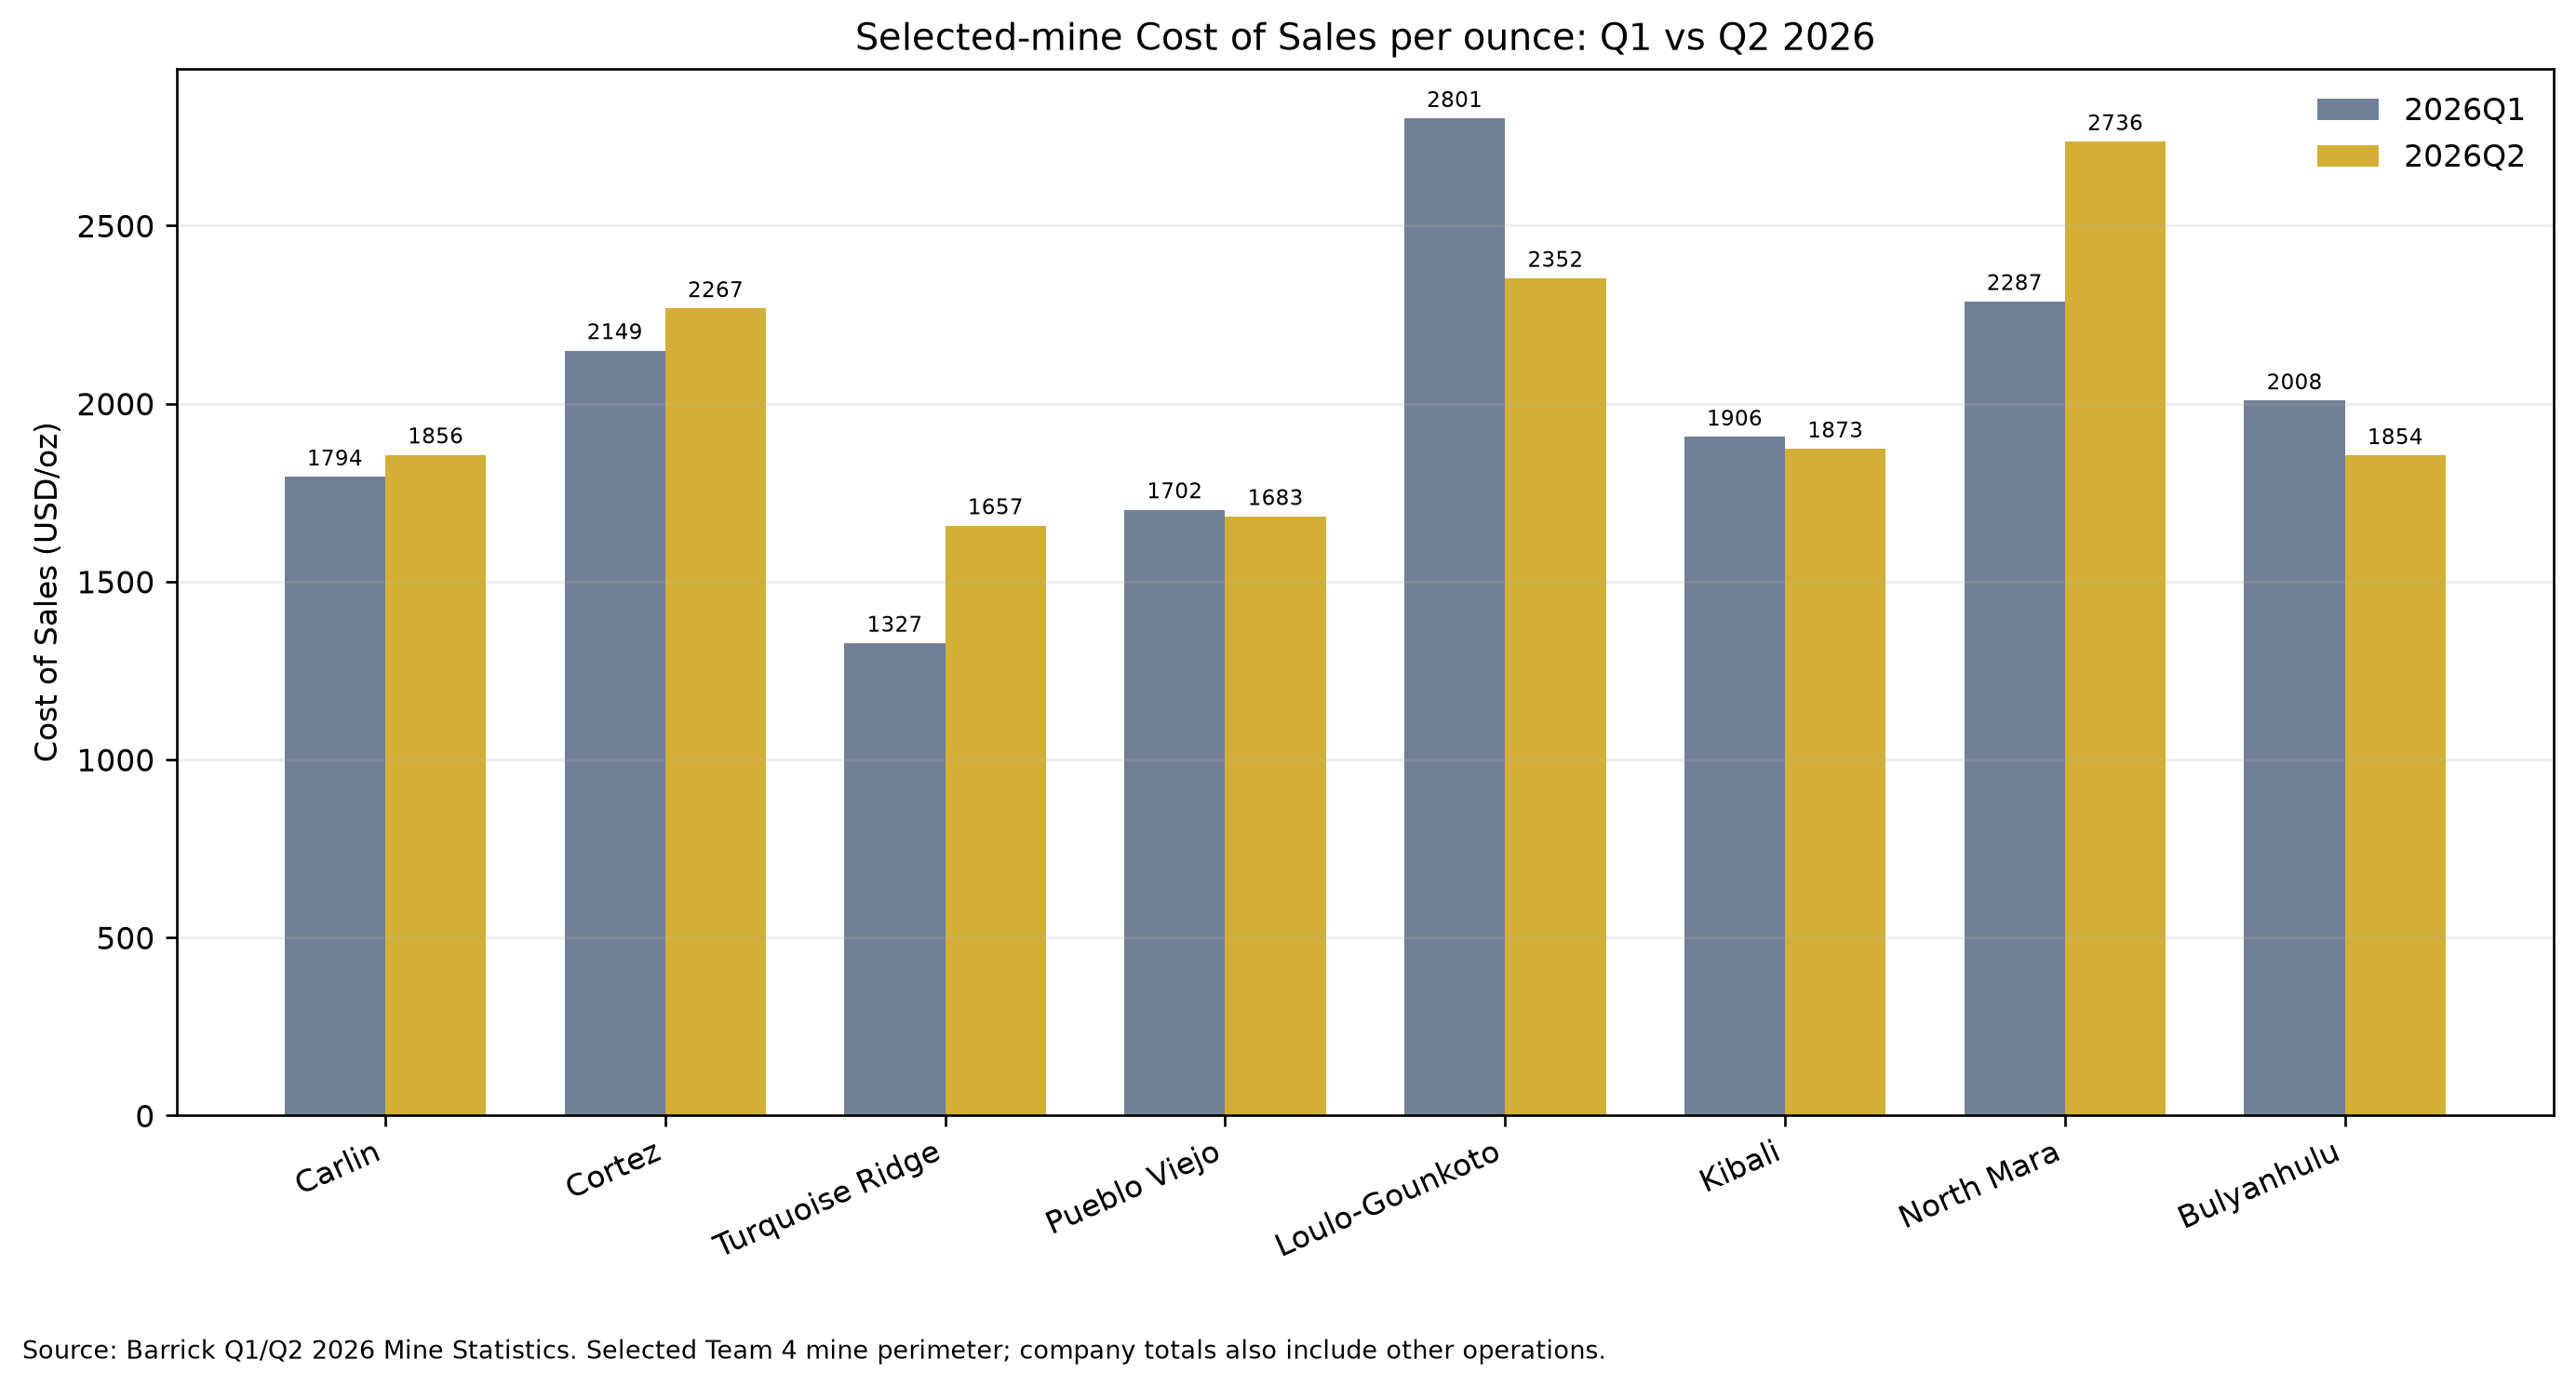
\includegraphics[width=0.95\columnwidth]{figures/team4_mine_cost_qoq.png}
  \captionof{figure}{Selected-mine Cost of Sales per ounce in Q1 and Q2 2026. Mine dispersion motivates preserving the Team 4 operating decomposition rather than replacing it with a single company-average cost.}
  \label{fig:team4_cost_qoq}
\par}

The refreshed actuals provide a transparent starting boundary for the operating forecast. From Q3 2026 onward, the unified experiment accepts the resulting deterministic 20-quarter cost vector rather than the fully stochastic CoS distributions explored in the source study. This design is intentional: simultaneous changes in gold, cost and production uncertainty would prevent clean attribution across the four price engines.

\subsection{Production block}
Production is modelled bottom-up rather than through a single total-output regression. Team 4 decomposes ounces into ore processed, average grade and recovery, using $SARIMA(1,0,1)(1,0,0)_4$ dynamics for ore, $SARIMA(1,0,0)(0,0,0)_4$ for grade and bounded stochastic simulation for recovery. The source does not report AIC/BIC selection for those production orders, so they are treated as admitted source specifications rather than re-selected models. Their physical recombination preserves mine heterogeneity and avoids the instability of a one-shot aggregate fit.

{\centering
  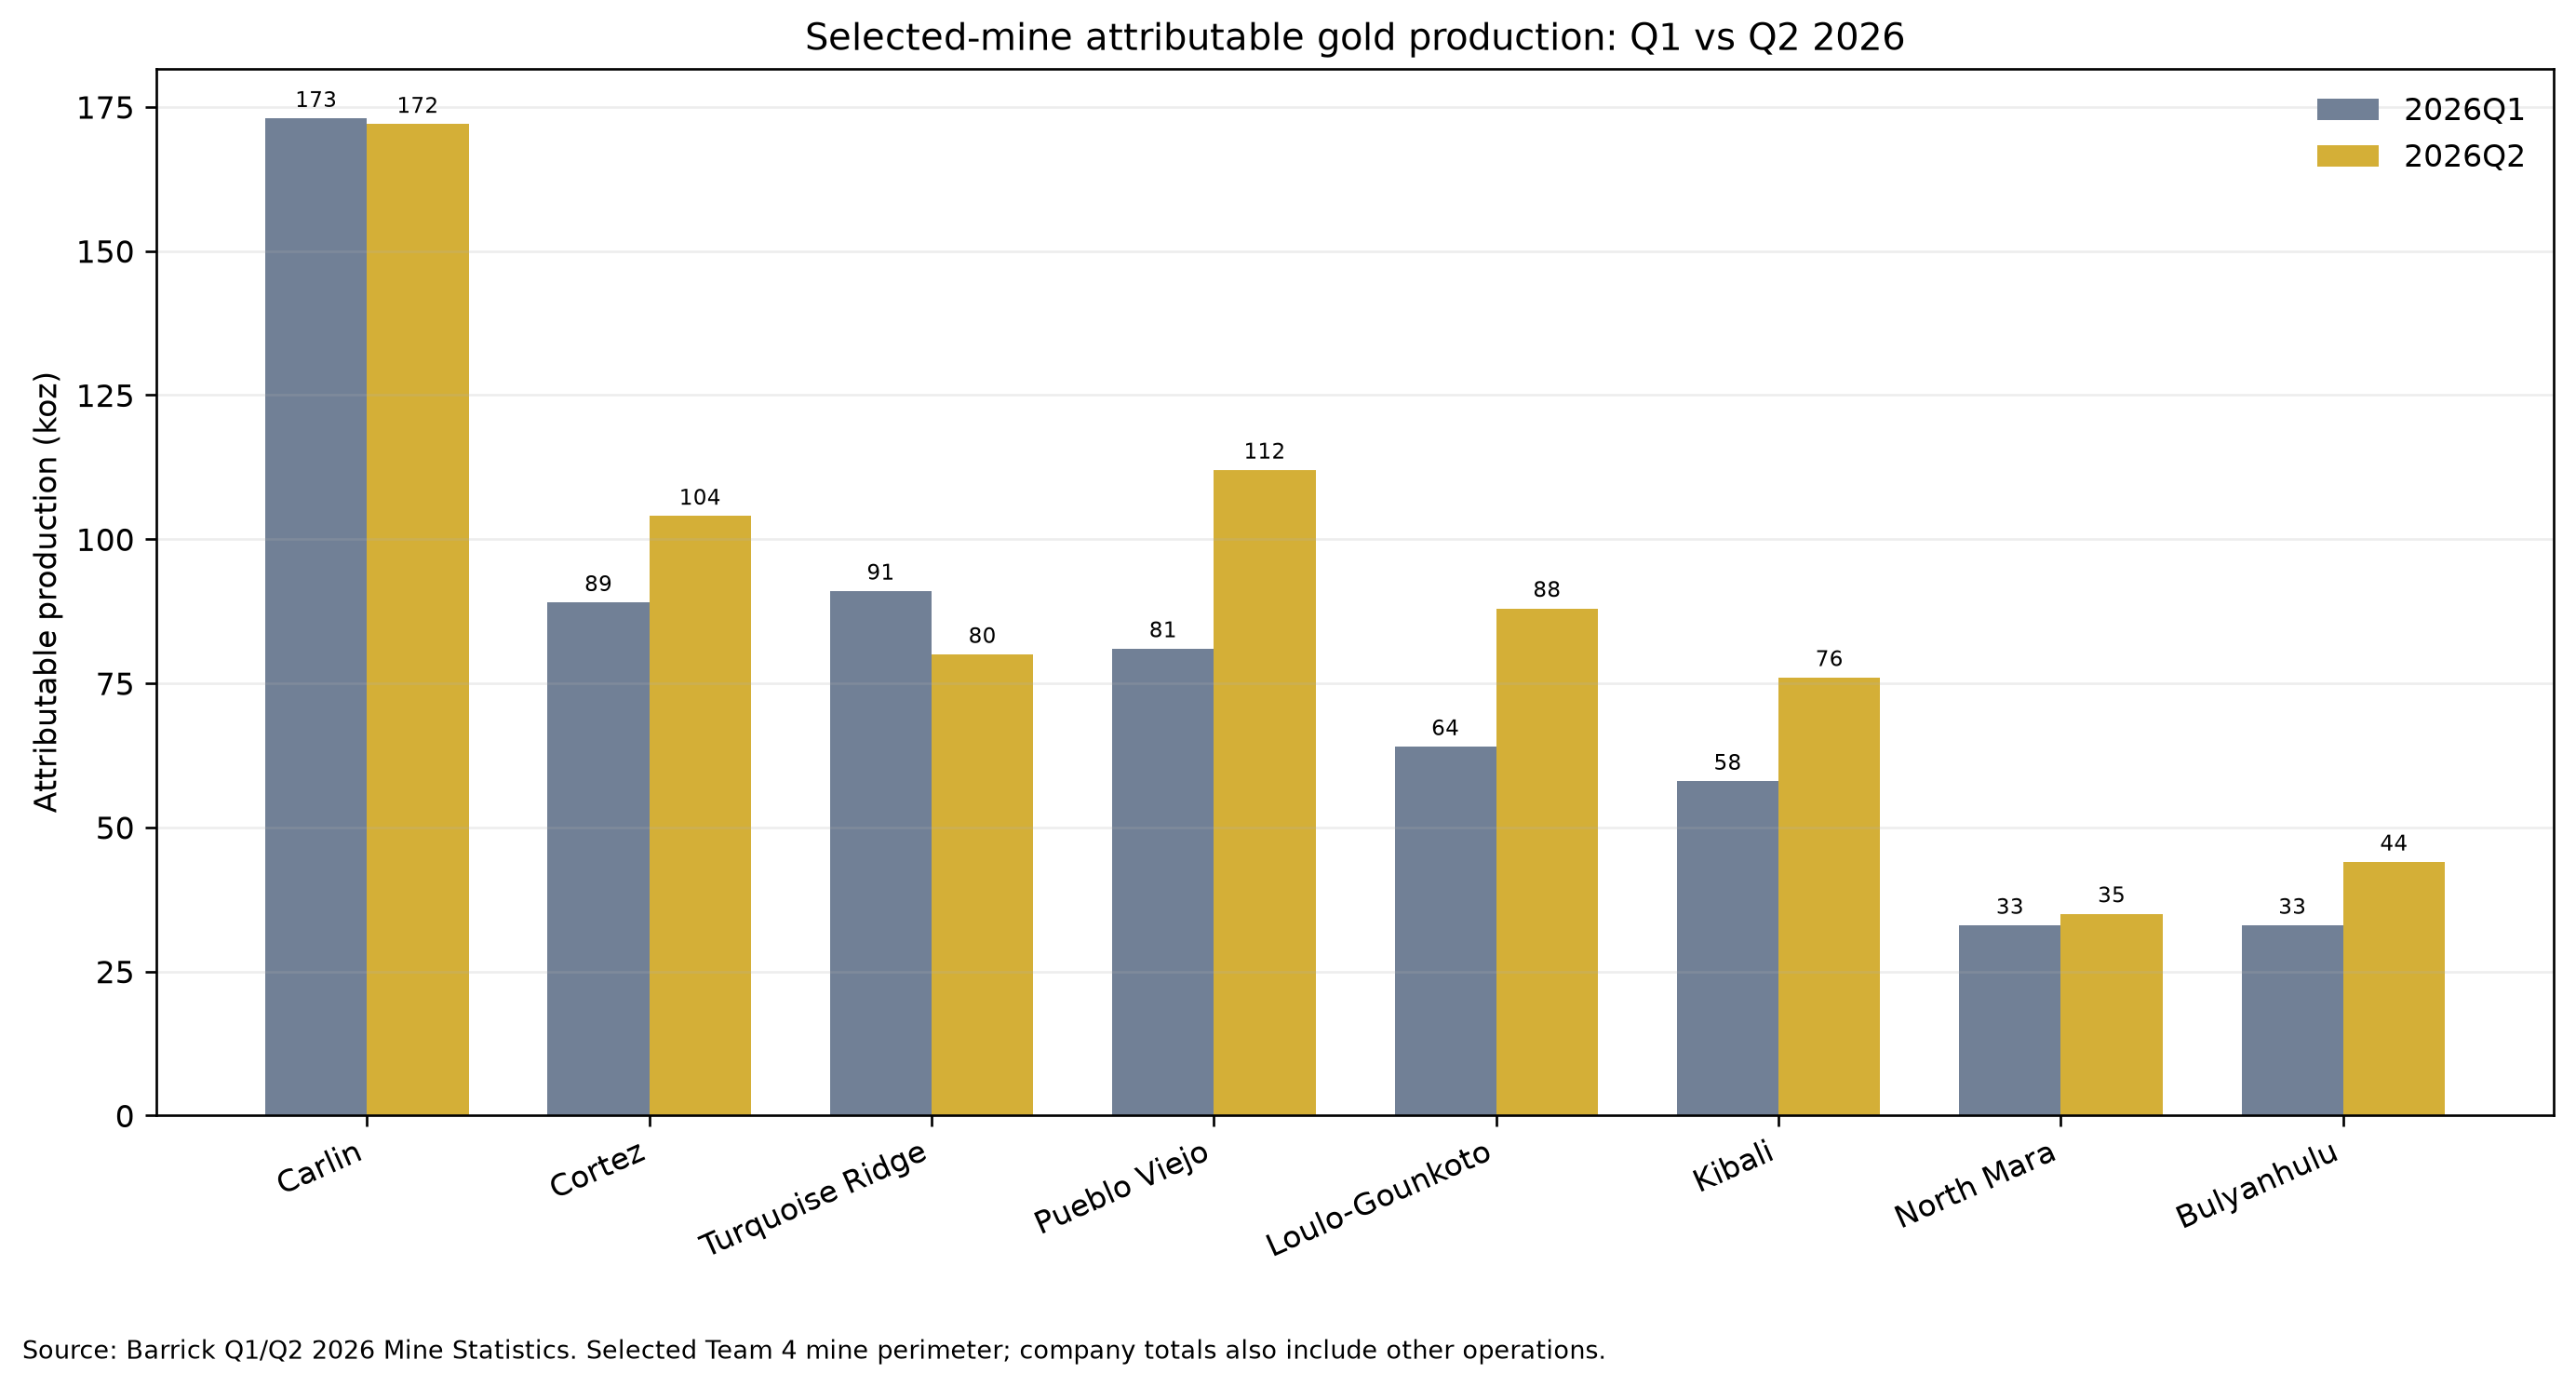
\includegraphics[width=0.95\columnwidth]{figures/team4_mine_production_qoq.png}
  \captionof{figure}{Selected-mine attributable gold production in Q1 and Q2 2026. The current actuals reveal heterogeneous changes that are hidden by a company-level total.}
  \label{fig:team4_production_qoq}
\par}

{\centering
  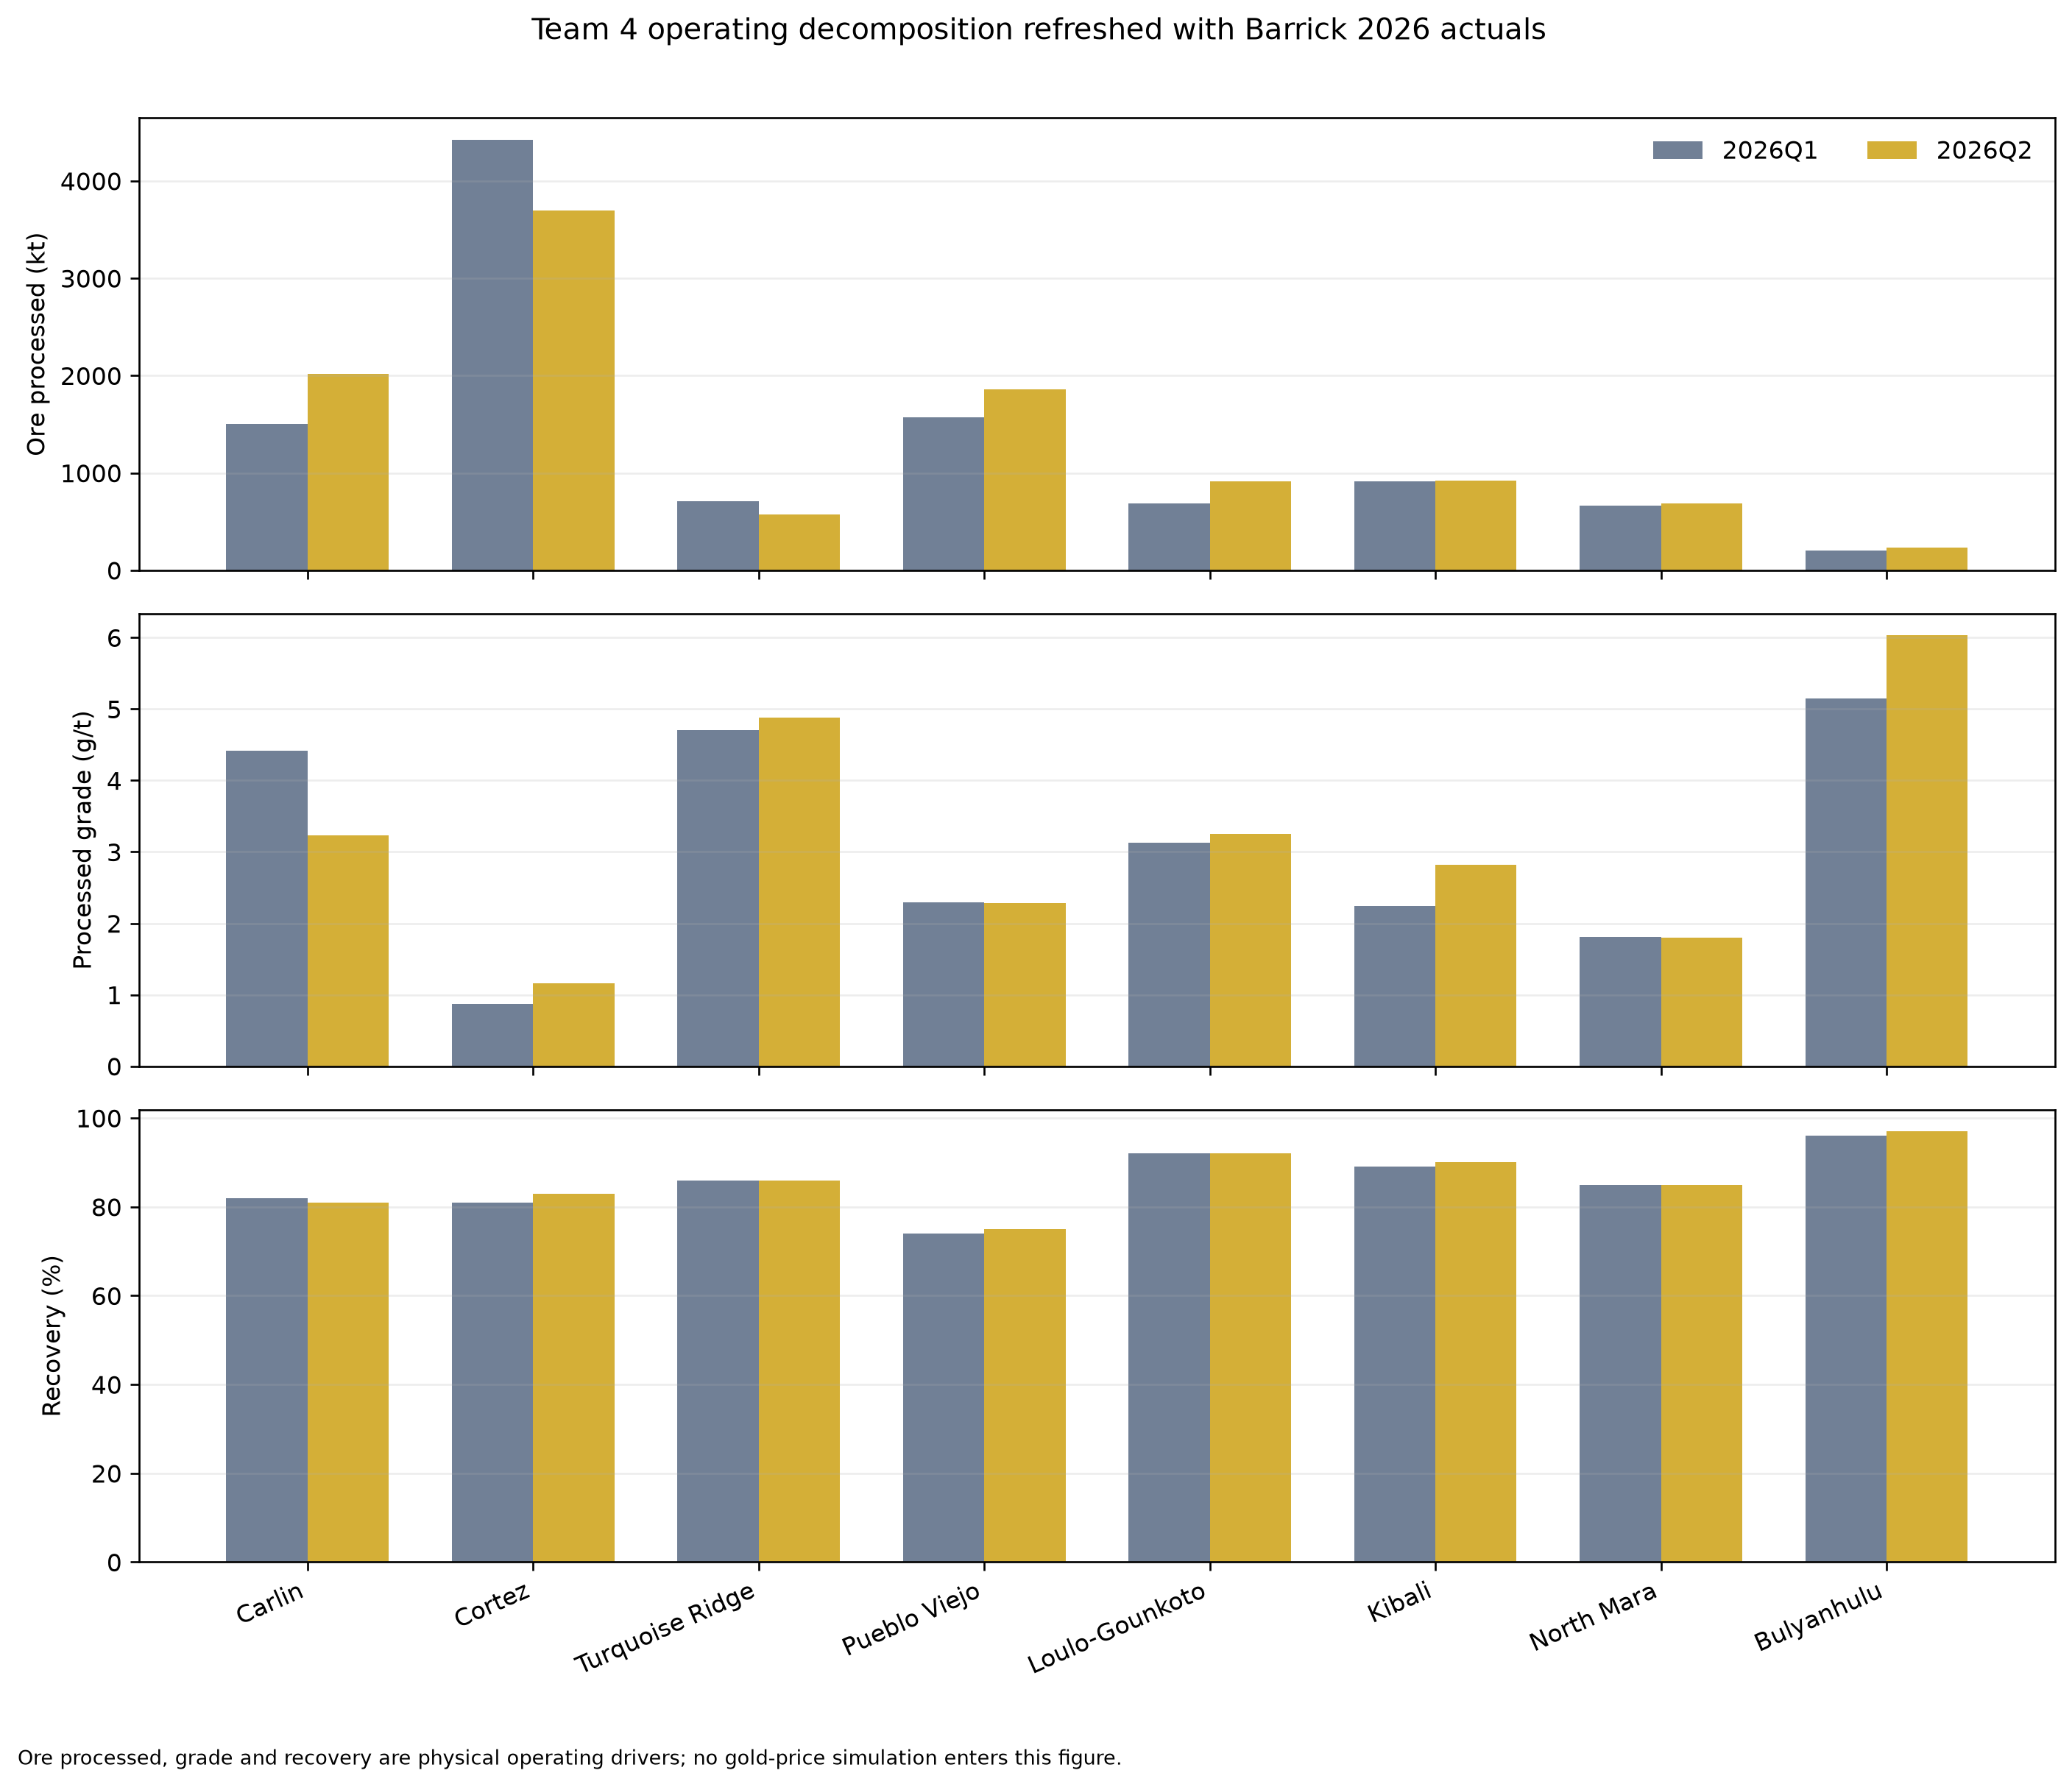
\includegraphics[width=0.95\columnwidth]{figures/team4_process_components_qoq.png}
  \captionof{figure}{Ore processed, grade and recovery updated with Barrick 2026 actuals. These are physical operating drivers; no commodity-price simulation enters the panel.}
  \label{fig:team4_process_qoq}
\par}

The original study also develops Goodman variance propagation and confidence bands for the production components. Those distributions remain useful evidence on operating-model uncertainty, but they are not propagated jointly in the four-engine corporate experiment: only the refreshed point vectors are passed downstream.

\subsection{Forecast handoff used by the valuation}
The final handoff keeps observed and modelled quantities distinct. Barrick's Q1--Q2 2026 actual production and CoS establish the current operating state; the Team 4 forecasts begin at Q3 2026 and extend through the common valuation horizon.

{\centering
  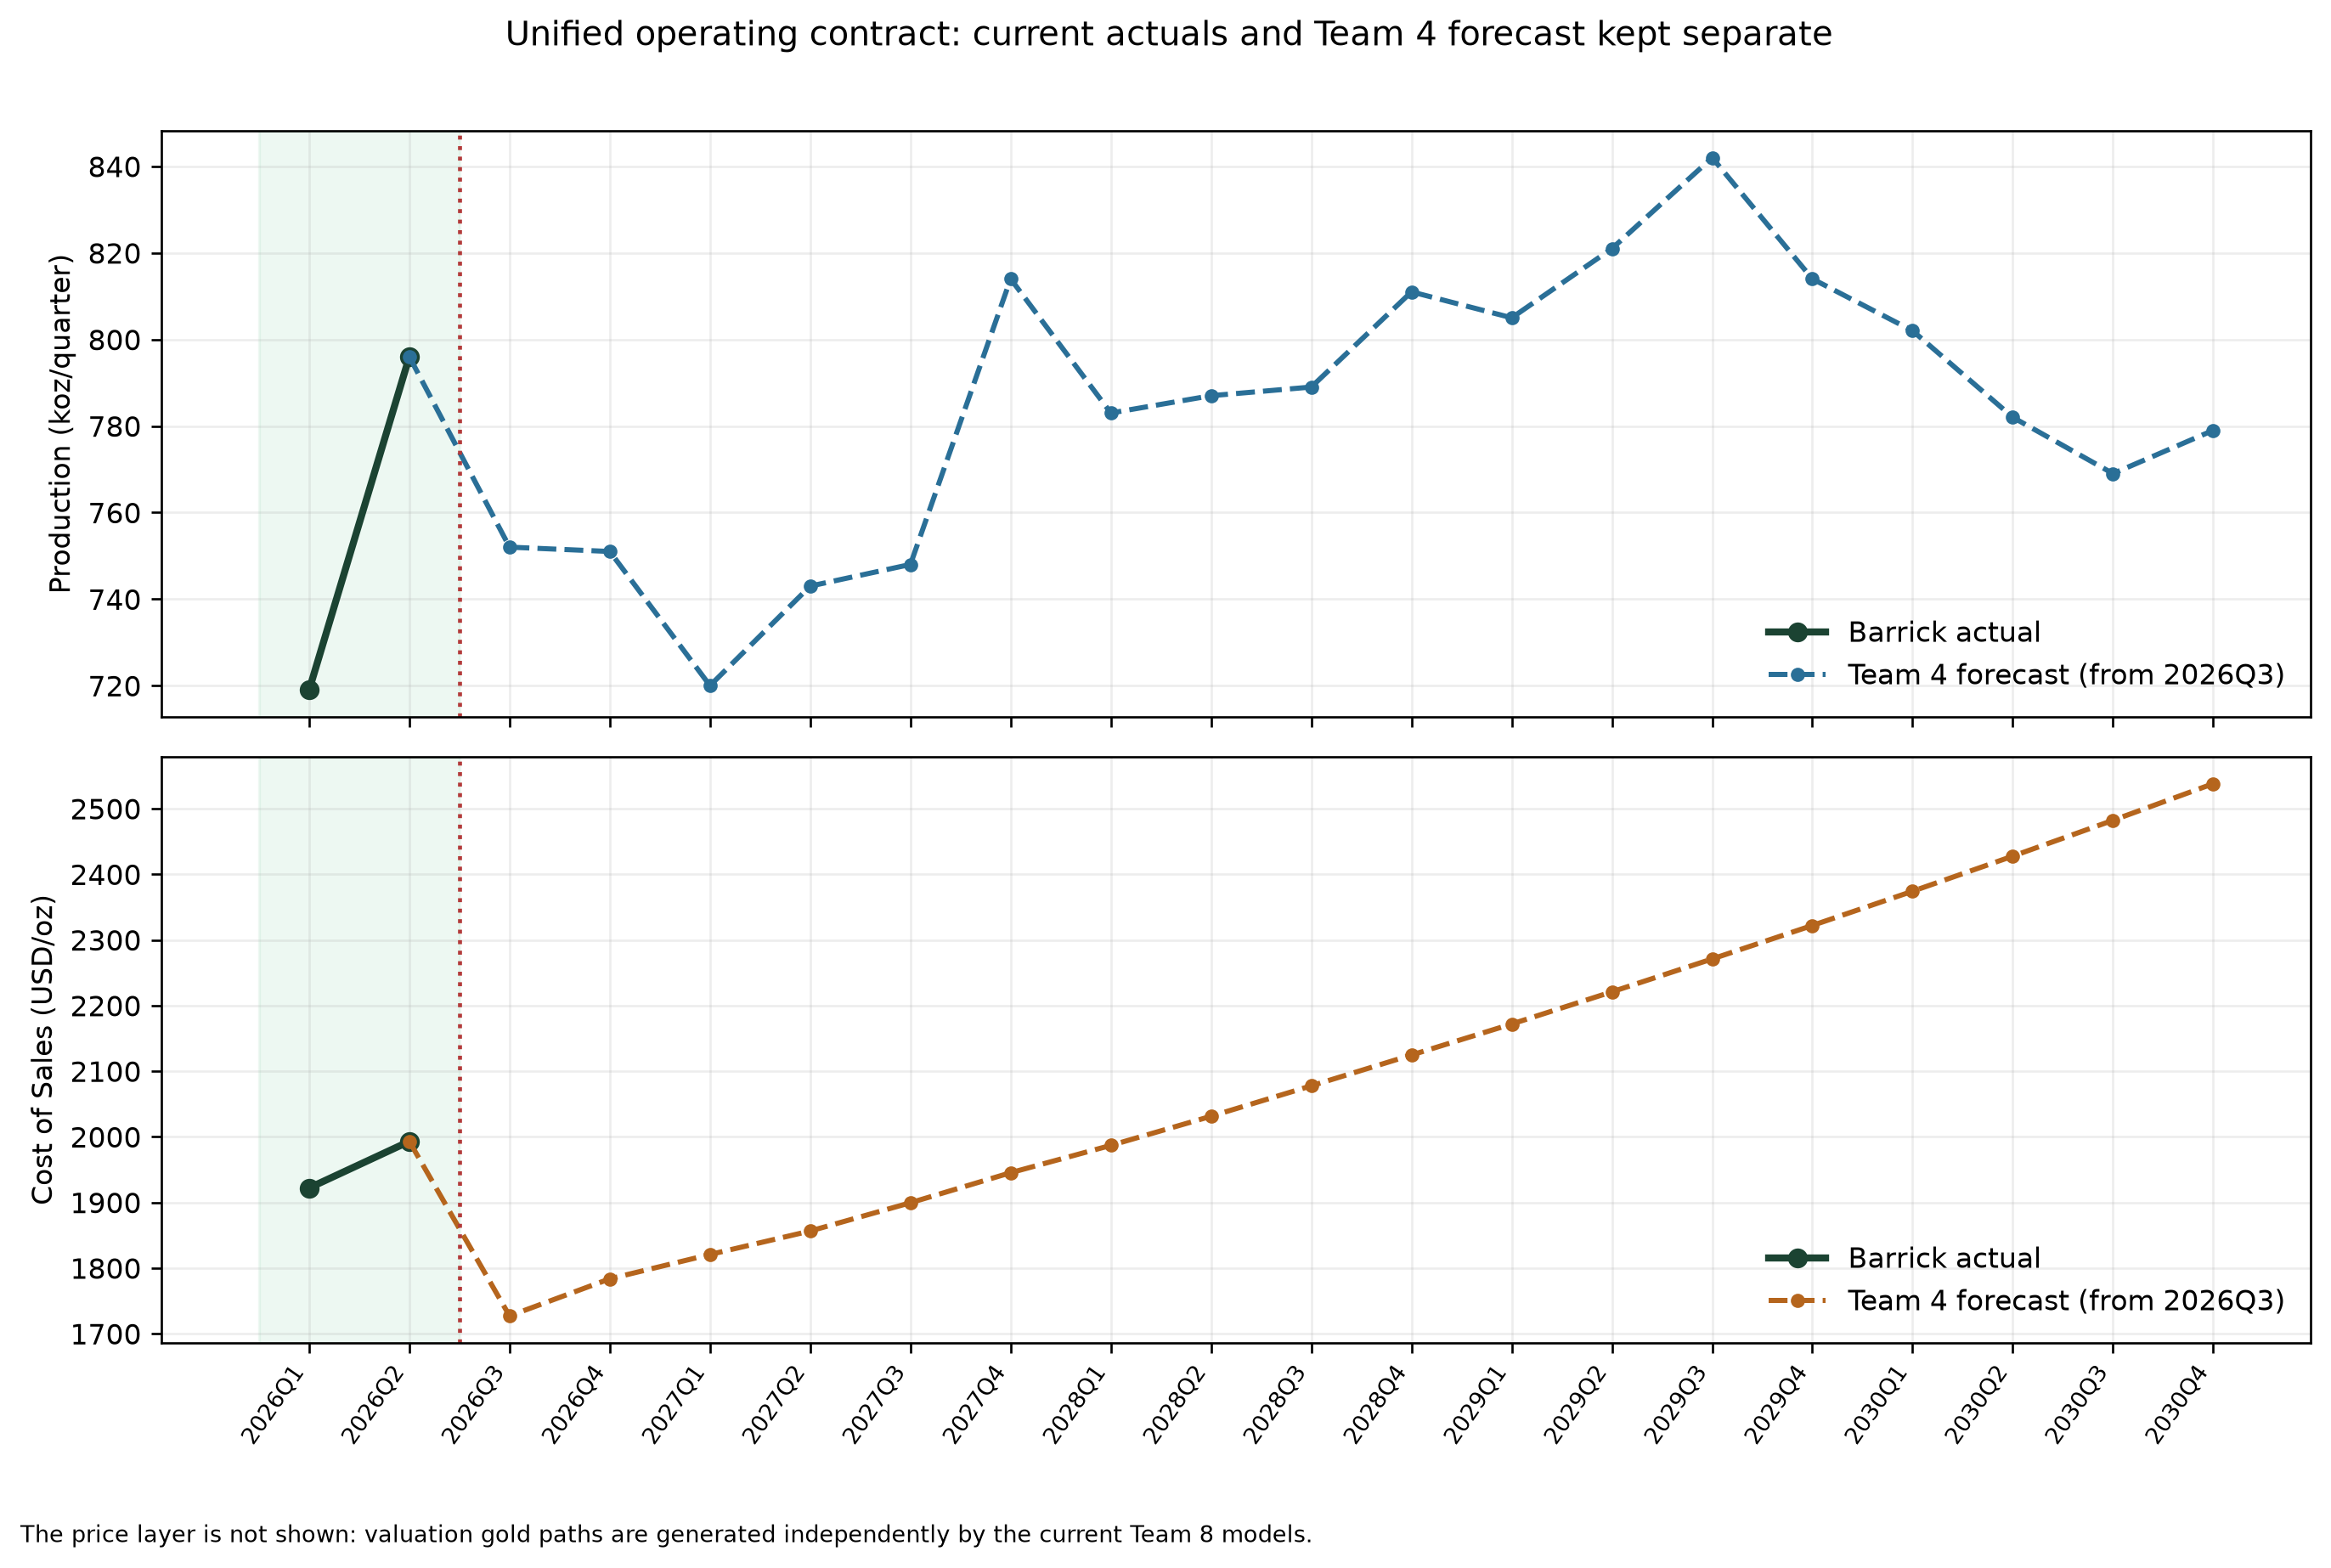
\includegraphics[width=0.95\columnwidth]{figures/team4_operating_contract.png}
  \captionof{figure}{Unified operating contract. Barrick Q1--Q2 2026 actuals are shown separately from the deterministic Team 4 production and CoS vectors used from Q3 2026 onward.}
  \label{fig:team4_contract}
\par}

\begin{methodbox}[Operating boundary]
The four valuation branches reuse the same refreshed production and cost vectors. Team 4's legacy gold-price and illustrative valuation outputs remain excluded, so differences in the final distributions can be attributed to the Team 8 gold-price process under a common Team 5 DCF contract.
\end{methodbox}

\section{Calibration Sample Audit}

{\centering
  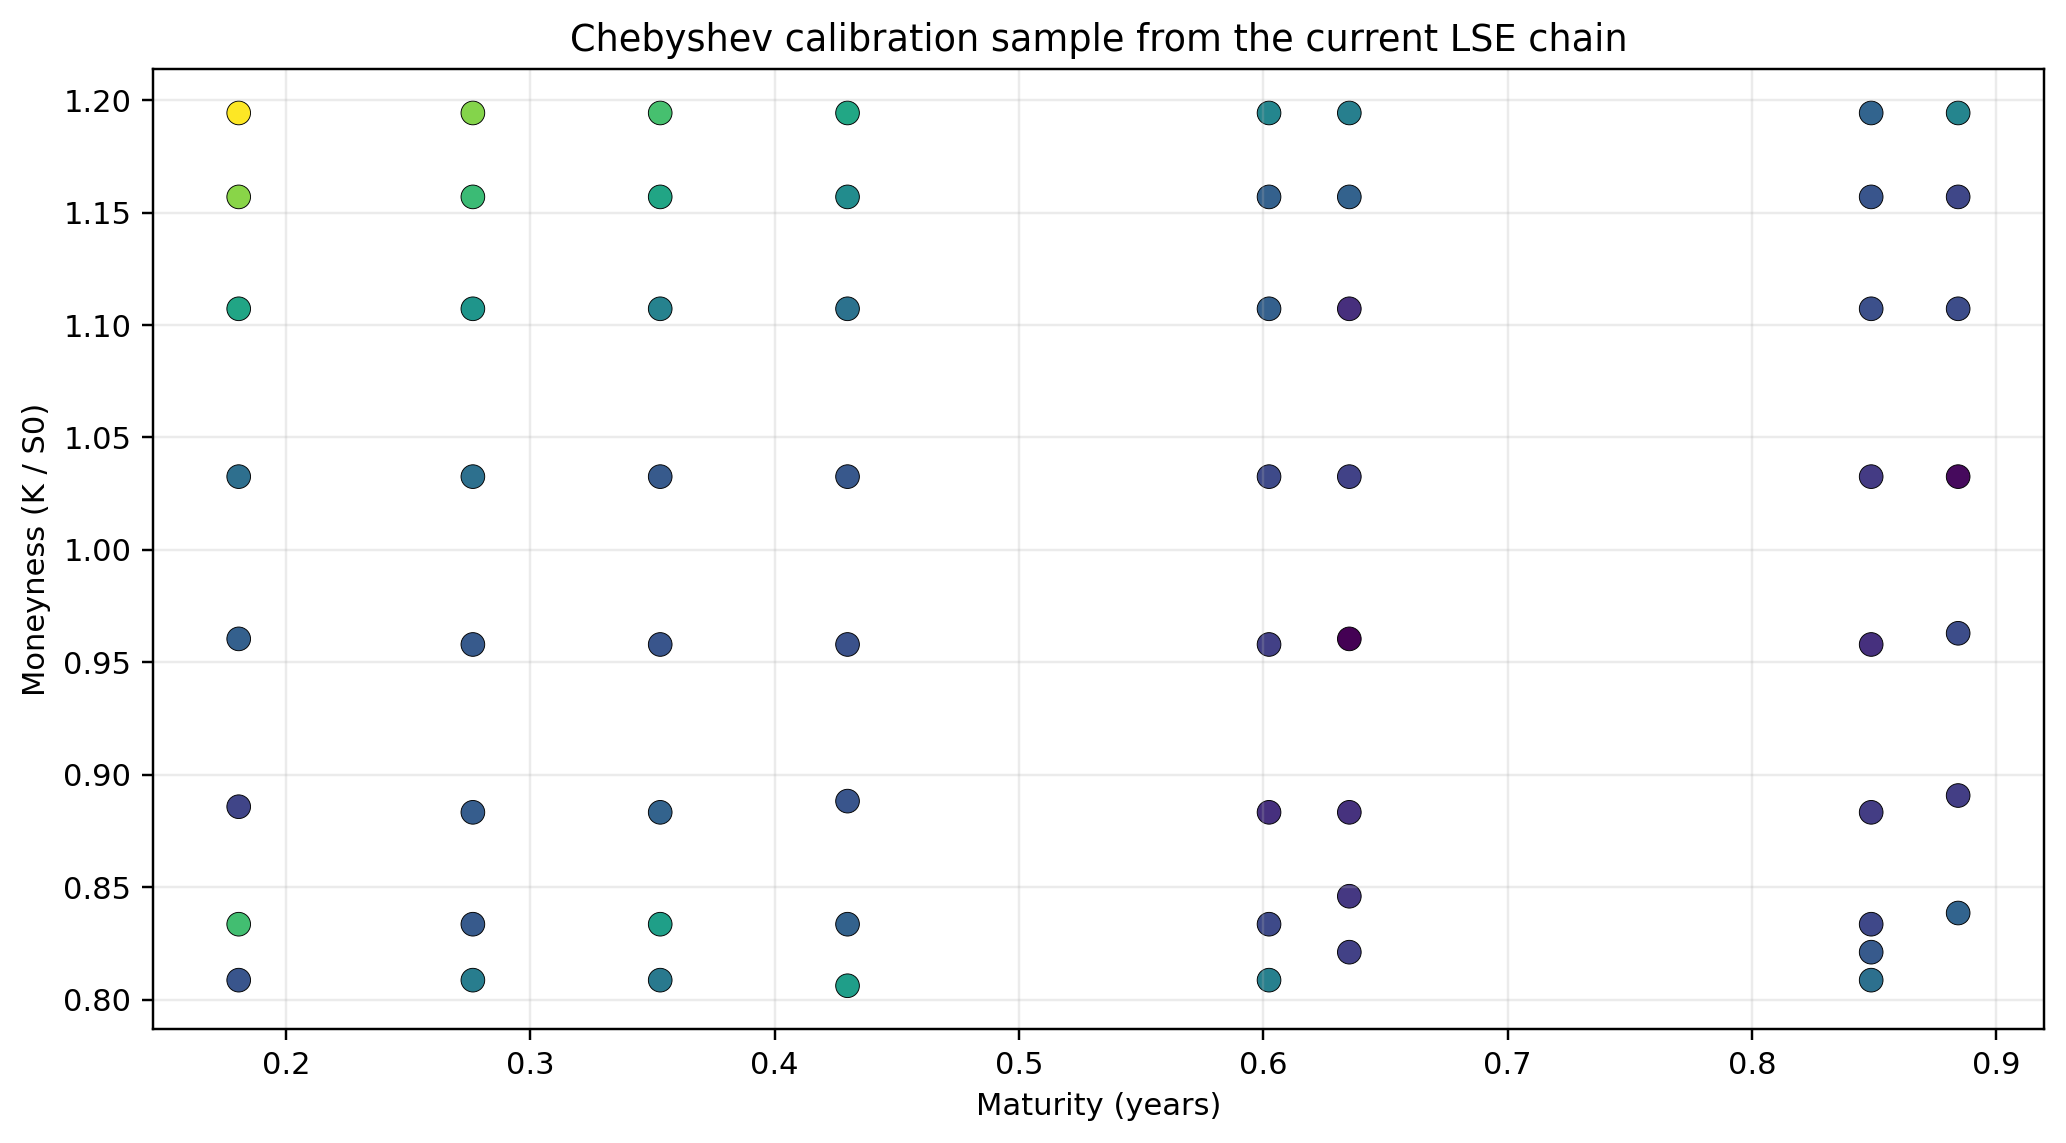
\includegraphics[width=0.95\columnwidth]{figures/sampling_comparison.png}
  \captionof{figure}{Final 2 September 2026 GLD surface and fixed CC64 geometry: 64 distinct actual contracts are selected from 605 eligible calls across 12 expiries and 146 strikes. Colour represents observed implied volatility.}
  \label{fig:chebyshev_audit}
\par}

\subsection{Why structured sampling is retained}
The option surface is irregular in strike and maturity. Team 8 therefore passes a fixed $8\times8$ Chebyshev--Chebyshev subset to the optimizer rather than allowing densely listed regions to dominate the loss. Every target is mapped to the nearest still-unused actual option: the 64-point calibration set contains no synthetic contracts. The figure audits the same 2 September parameter snapshot used by the refreshed valuation.

\begin{methodbox}[Evidence status]
The calibrated inputs, residual maps and valuation paths share the same 2 September Team 8 parameter set. The U.S. Treasury curve is dated 2 September as well; the separate Q2 realized-gold level anchor remains explicit in the valuation contract.
\end{methodbox}

\subsection{What the residual maps add}
The residual heatmaps show where each specification systematically over- or under-prices the observed implied-volatility surface. Black--Scholes leaves the strongest smile and term-structure pattern. On this snapshot Heston provides the lowest IV RMSE at 49.4881 bp; Full Bates--Hawkes follows at 52.9714 bp and Bates at 54.6273 bp. The fitted Hawkes branching ratio is 0.5569, below the stationarity boundary but economically material. The four maps are arranged as a two-by-two comparison so their common axes and colour scales remain directly comparable.

\end{multicols}

\vspace{4pt}
{\centering
\begin{minipage}[t]{0.485\textwidth}
  \centering
  
\includegraphics[width=\linewidth]{figures/black_scholes_residual_heatmap.png}
  \par\vspace{1pt}{\footnotesize\textbf{(a)} Black--Scholes\par}
\end{minipage}\hfill%
\begin{minipage}[t]{0.485\textwidth}
  \centering
  
\includegraphics[width=\linewidth]{figures/heston_residual_heatmap.png}
  \par\vspace{1pt}{\footnotesize\textbf{(b)} Heston\par}
\end{minipage}

\vspace{2pt}

\begin{minipage}[t]{0.485\textwidth}
  \centering
  
\includegraphics[width=\linewidth]{figures/bates_residual_heatmap.png}
  \par\vspace{1pt}{\footnotesize\textbf{(c)} Bates--Poisson\par}
\end{minipage}\hfill%
\begin{minipage}[t]{0.485\textwidth}
  \centering
  
\includegraphics[width=\linewidth]{figures/bates_hawkes_residual_heatmap.png}
  \par\vspace{1pt}{\footnotesize\textbf{(d)} Full Bates--Hawkes\par}
\end{minipage}
\captionof{figure}{Implied-volatility residual maps for the common 2 September CC64 sample. Blue denotes model IV above market IV and red denotes model IV below market; Heston records the lowest in-sample IV RMSE.}
\label{fig:residual_maps}
}
\vspace{4pt}

\begin{multicols}{2}
\raggedcolumns

\section{DCF Driver and Terminal-Value Audit}

Growth, reinvestment, WACC and terminal closure are shared across gold engines. Table~\ref{tab:dcf_inputs} summarizes the corporate assumptions.

\subsection{Growth, ROIC and reinvestment}
Growth and ROIC converge linearly to their stable levels over five years. Reinvestment follows $b_t=g_t/ROIC_t$, linking growth to the capital required to sustain it (Figure~\ref{fig:dcf_driver_schedule}).

\noindent\begin{minipage}{\columnwidth}
{\centering
  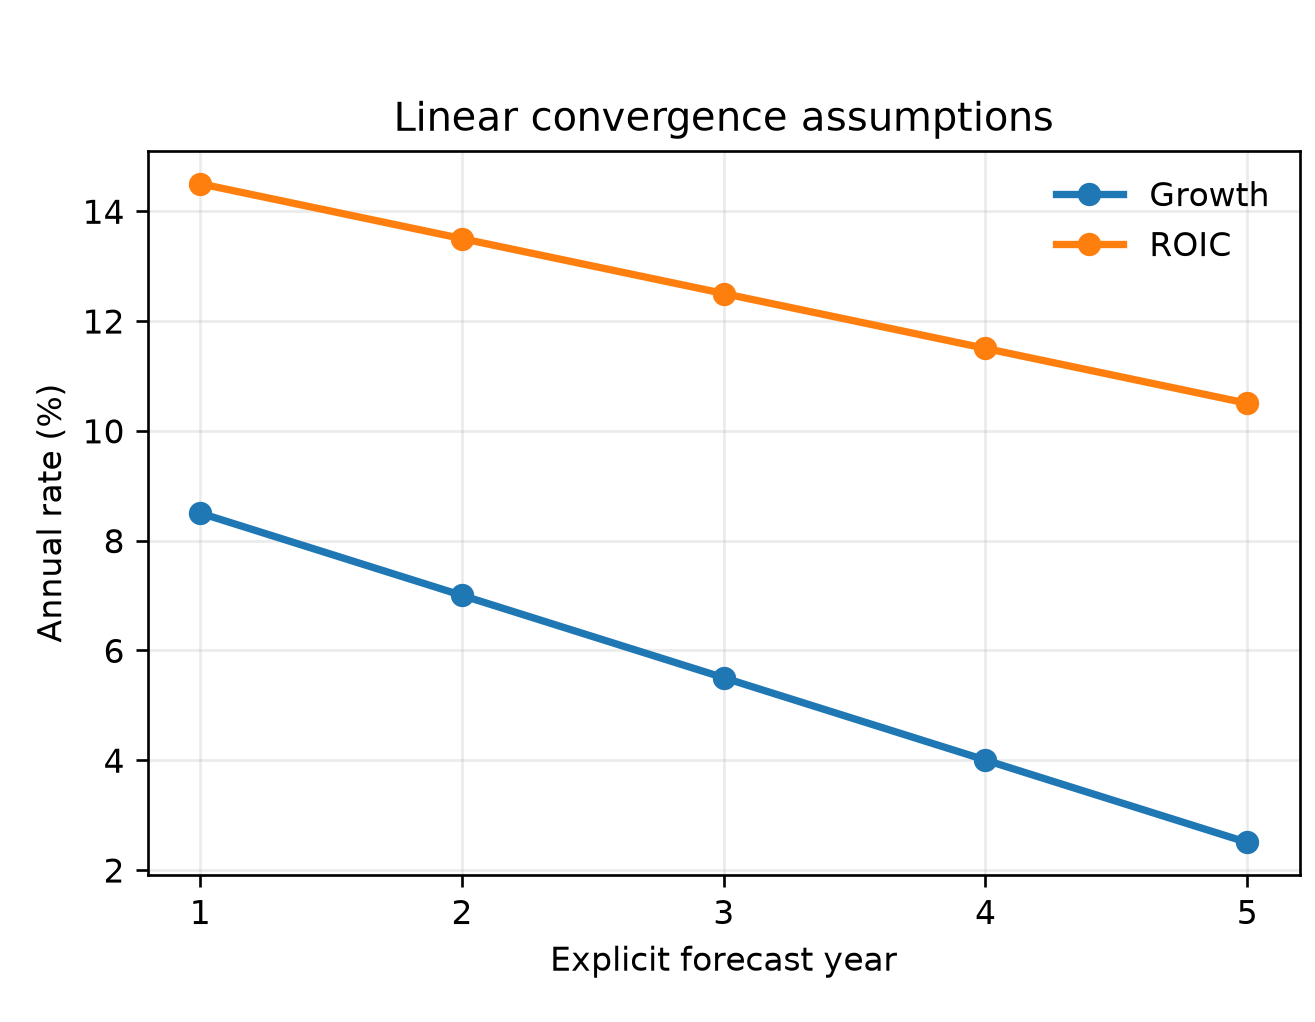
\includegraphics[width=0.90\linewidth]{figures/fig_dcf_growth_roic.png}
  \captionof{figure}{Common explicit-period DCF schedule: growth and ROIC converge linearly over the five-year horizon.}
  \label{fig:dcf_driver_schedule}
\par}
\end{minipage}\par

\noindent\begin{minipage}{\columnwidth}
{\centering
  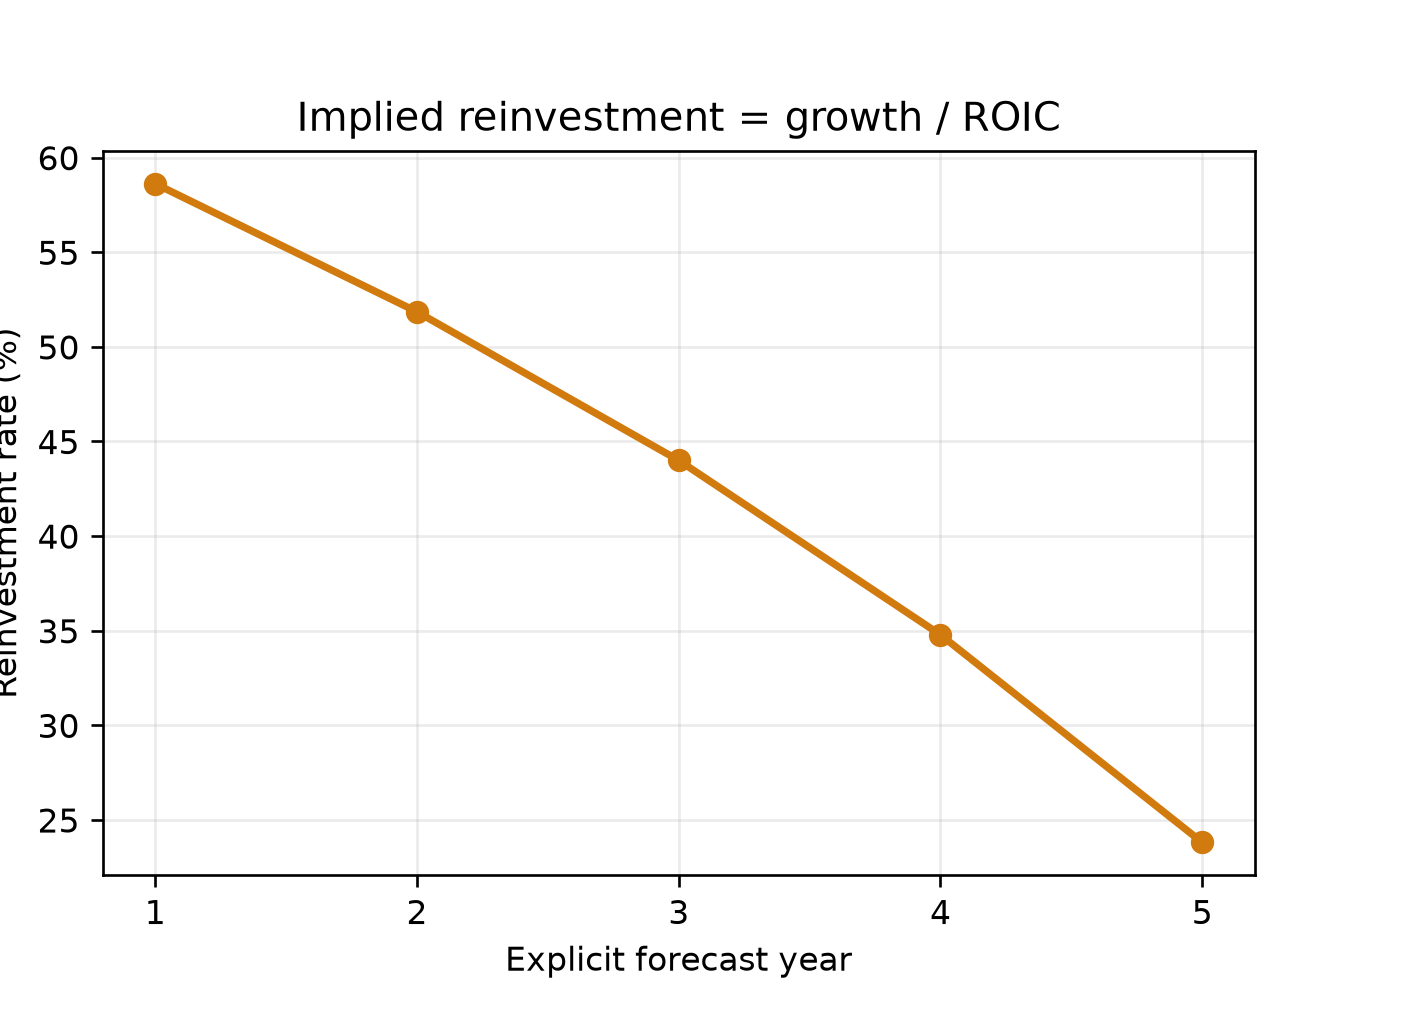
\includegraphics[width=0.90\linewidth]{figures/fig_dcf_reinvestment.png}
  \captionof*{figure}{\textbf{Figure~\ref{fig:dcf_driver_schedule} (continued).} The implied reinvestment rate, defined as growth divided by ROIC, falls from 58.62\% to 23.81\%.}
\par}
\end{minipage}\par

\subsection{Common stochastic WACC}
WACC follows the bounded mean-reverting process in Equation~(17), with inputs in Table~\ref{tab:dcf_inputs}. Its annual conditional standard deviation is 0.7308 percentage points. All branches reuse the same 8,192-path shock array; Figure~\ref{fig:wacc_assumptions} shows its distribution and zero-shock path.

\noindent\begin{minipage}{\columnwidth}
{\centering
  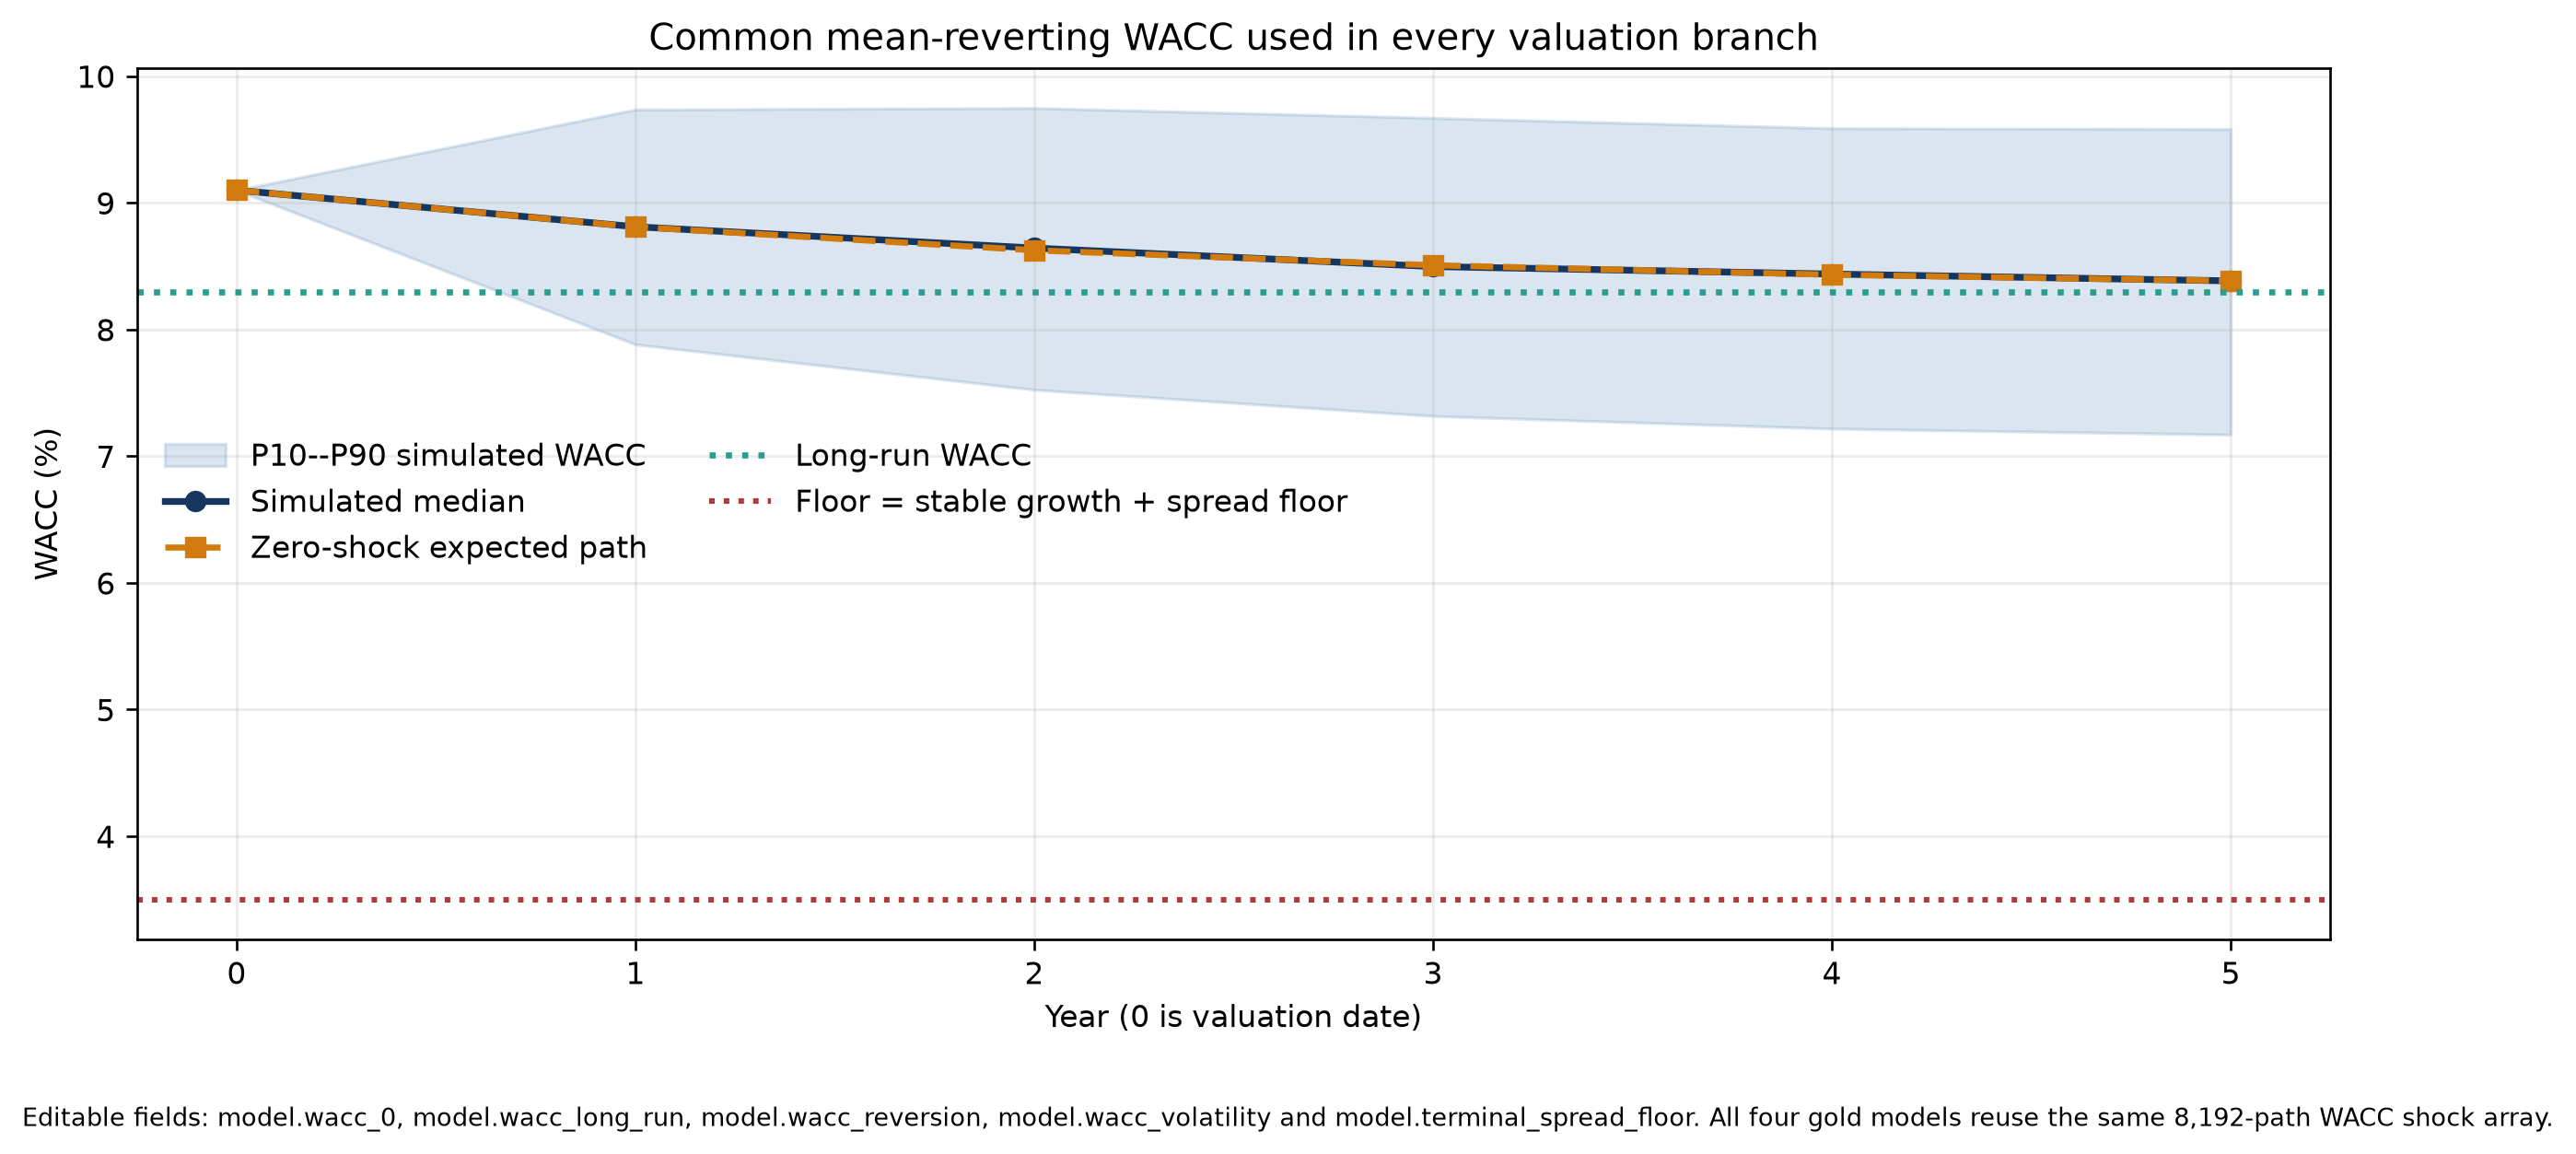
\includegraphics[width=0.95\columnwidth]{figures/fig_wacc_assumptions.png}
  \captionof{figure}{Common mean-reverting WACC. The band is the P10--P90 range from the shared 8,192-path shock array; the orange line is the zero-shock path and the dotted lines show the long-run level and admissibility floor.}
  \label{fig:wacc_assumptions}
\par}
\end{minipage}\par

\subsection{Terminal closure and sensitivity}
The terminal block uses $g_\infty=2.50\%$, $ROIC_\infty=10.50\%$ and terminal reinvestment of 23.81\%. At the current median terminal WACC of 8.384\%, the normalized terminal multiple is 13.27$\times$ final after-tax margin. The denominator is admitted only when $WACC_T>g_\infty$; the spread floor prevents a mechanically explosive closure in the simulated paths.

\noindent\begin{minipage}{\columnwidth}
{\centering
  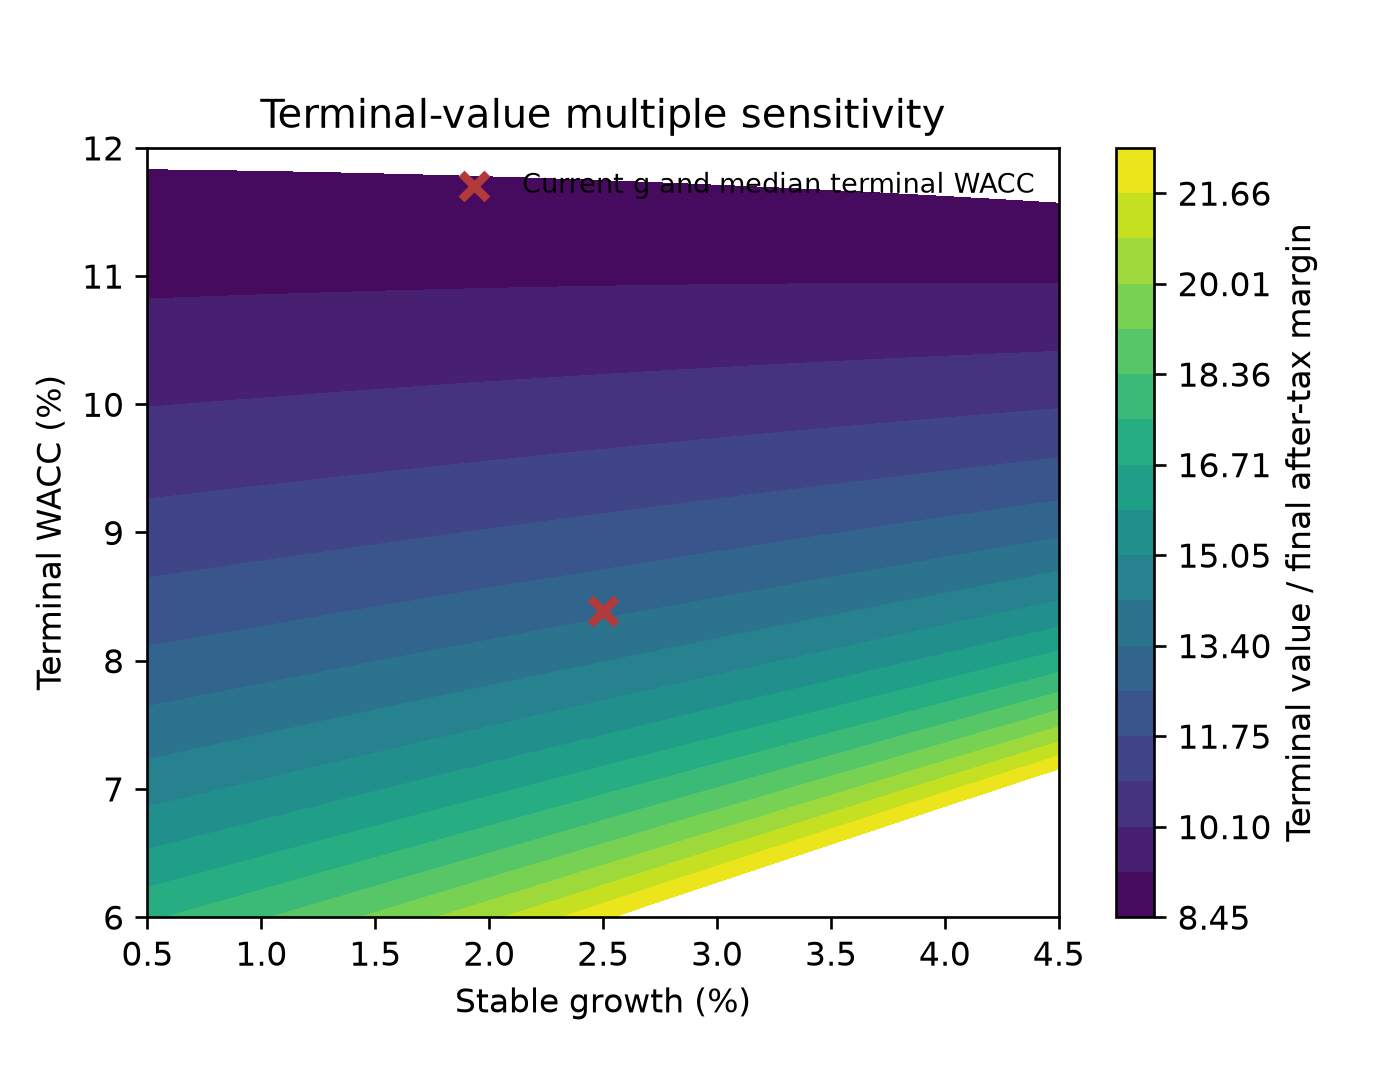
\includegraphics[width=0.90\linewidth]{figures/fig_terminal_multiple.png}
  \captionof{figure}{Terminal-value multiple sensitivity to stable growth and terminal WACC. The cross marks the configured stable-growth rate and current median terminal WACC.}
  \label{fig:terminal_value_mechanics}
\par}
\end{minipage}\par

\noindent\begin{minipage}{\columnwidth}
{\centering
  
\includegraphics[width=0.90\linewidth]{figures/fig_terminal_share.png}
  \captionof*{figure}{\textbf{Figure~\ref{fig:terminal_value_mechanics} (continued).} Present-value terminal share on positive-EV paths. Refreshed medians are 78.26\% for Black--Scholes, 78.31\% for Heston, 78.43\% for Bates and 78.27\% for Full Bates--Hawkes; bars show the P10--P90 range.}
\par}
\end{minipage}\par

\begin{table}[H]
\centering
\caption{Editable common DCF inputs.}
\label{tab:dcf_inputs}
\begin{tabularx}{\columnwidth}{@{}Xr@{}}
\toprule
Parameter & Value \\
\midrule
Tax rate & 25.00\% \\
$g_1\rightarrow g_\infty$ & 8.50--2.50\% \\
$ROIC_1\rightarrow ROIC_\infty$ & 14.50--10.50\% \\
$WACC_0\rightarrow\bar w$ & 9.10--8.30\% \\
WACC reversion & 0.45 \\
WACC volatility & 0.90\% \\
WACC floor/cap & 3.50/25.00\% \\
Terminal reinvestment & 23.81\% \\
\bottomrule
\end{tabularx}
\end{table}

\begin{methodbox}[Interpretation]
These are transparent methodological assumptions, not filing-calibrated Barrick estimates. Their materiality is visible: the terminal block supplies roughly three quarters of positive enterprise value. They should therefore be changed centrally and sensitivity-tested rather than hidden inside a single headline valuation.
\end{methodbox}

\section{Operating-Proxy Sensitivities}

\begin{table}[H]
\centering
\caption{Audited Bates--Hawkes operating proxy.}
\label{tab:primary_signal}
\begin{tabularx}{\columnwidth}{@{}Xr@{}}
\toprule
Metric & USD billion or \% \\
\midrule
P10 & 1.03 \\
Median (P50) & 59.82 \\
P90 & 172.60 \\
Mean & 77.95 \\
Negative proxy paths & 9.30\% \\
Five-year-only median & 12.89 \\
Legacy floor mean uplift & 1.49 \\
\bottomrule
\end{tabularx}
\end{table}

\begin{findingbox}[Interpretation]
These are unconstrained aggregate operating proxies, not enterprise or equity values. The Q-law/WACC combination has no demonstrated corporate pricing interpretation. Negative outcomes are not negative limited-liability share prices; no market comparison is made.
\end{findingbox}

\noindent\begin{minipage}{\columnwidth}
{\centering
  
\includegraphics[width=0.95\columnwidth]{figures/fig_val_primary.png}
  \captionof{figure}{Signed-terminal operating proxy under audited Bates--Hawkes parameters. The common contract is reused across 8,192 paths. Display limits are the 0.5th--99.5th percentiles; the full tails remain in the data. This is not a confidence interval or physical probability law.}
  \label{fig:value_distribution}
\par}
\end{minipage}\par

\subsection{Cross-model central tendency}
Audited parameter refinements dated 7 September use the unchanged 2 September market sample. Cross-model medians range from USD 59.12 to 60.10 billion and P90 from USD 172.60 to 174.02 billion. Their proximity should not be interpreted as a robust ranking of companies or models.

\begin{table}[H]
\centering
\caption{Aggregate proxy medians, USD billion.}
\label{tab:model_comparison}
\begin{tabular}{@{}lrr@{}}
\toprule
Gold engine & Median & Five-year only \\
\midrule
Black--Scholes & 60.10 & 13.17 \\
Heston & 59.77 & 13.08 \\
Bates--Poisson & 59.12 & 12.83 \\
Full Bates--Hawkes & 59.82 & 12.89 \\
\bottomrule
\end{tabular}
\end{table}

% Expansion p6 - 2026-09-06
The simulation spread describes conditional scenario dispersion; Monte Carlo error concerns numerical estimates. Doubling paths to 16,384, doubling fine steps to 520 and changing the seed gives Bates--Hawkes medians of 59.34, 61.59 and 61.38 billion versus 59.82 at baseline. Such numerical variation exceeds some cross-model median gaps. Negative values expose the unconstrained mapping, not negative limited-liability shares. The data retain these outcomes rather than silently flooring them.

\subsection{Structural illustration, not model selection}
Bates--Hawkes illustrates the richest law, not a preferred corporate valuation. Its audited branching ratio is 0.5594 and kernel half-life $\log(2)/\beta=0.2522$ years. These are risk-neutral fitted parameters, not measured geopolitical persistence. The earlier OOS exercise below uses the original, unrefined origin fits.

\noindent\begin{minipage}{\columnwidth}
{\centering
  
\includegraphics[width=0.95\columnwidth]{figures/fig_val_multi.png}
  \captionof{figure}{Audited operating-proxy distributions under four gold-price laws. Operations, WACC and signed terminal closure are common. No share count, equity bridge or market reference is used.}
  \label{fig:multimodel_value_overlay}
\par}
\end{minipage}\par

\section{Out-of-Sample Evidence and Model Risk}

{\centering
  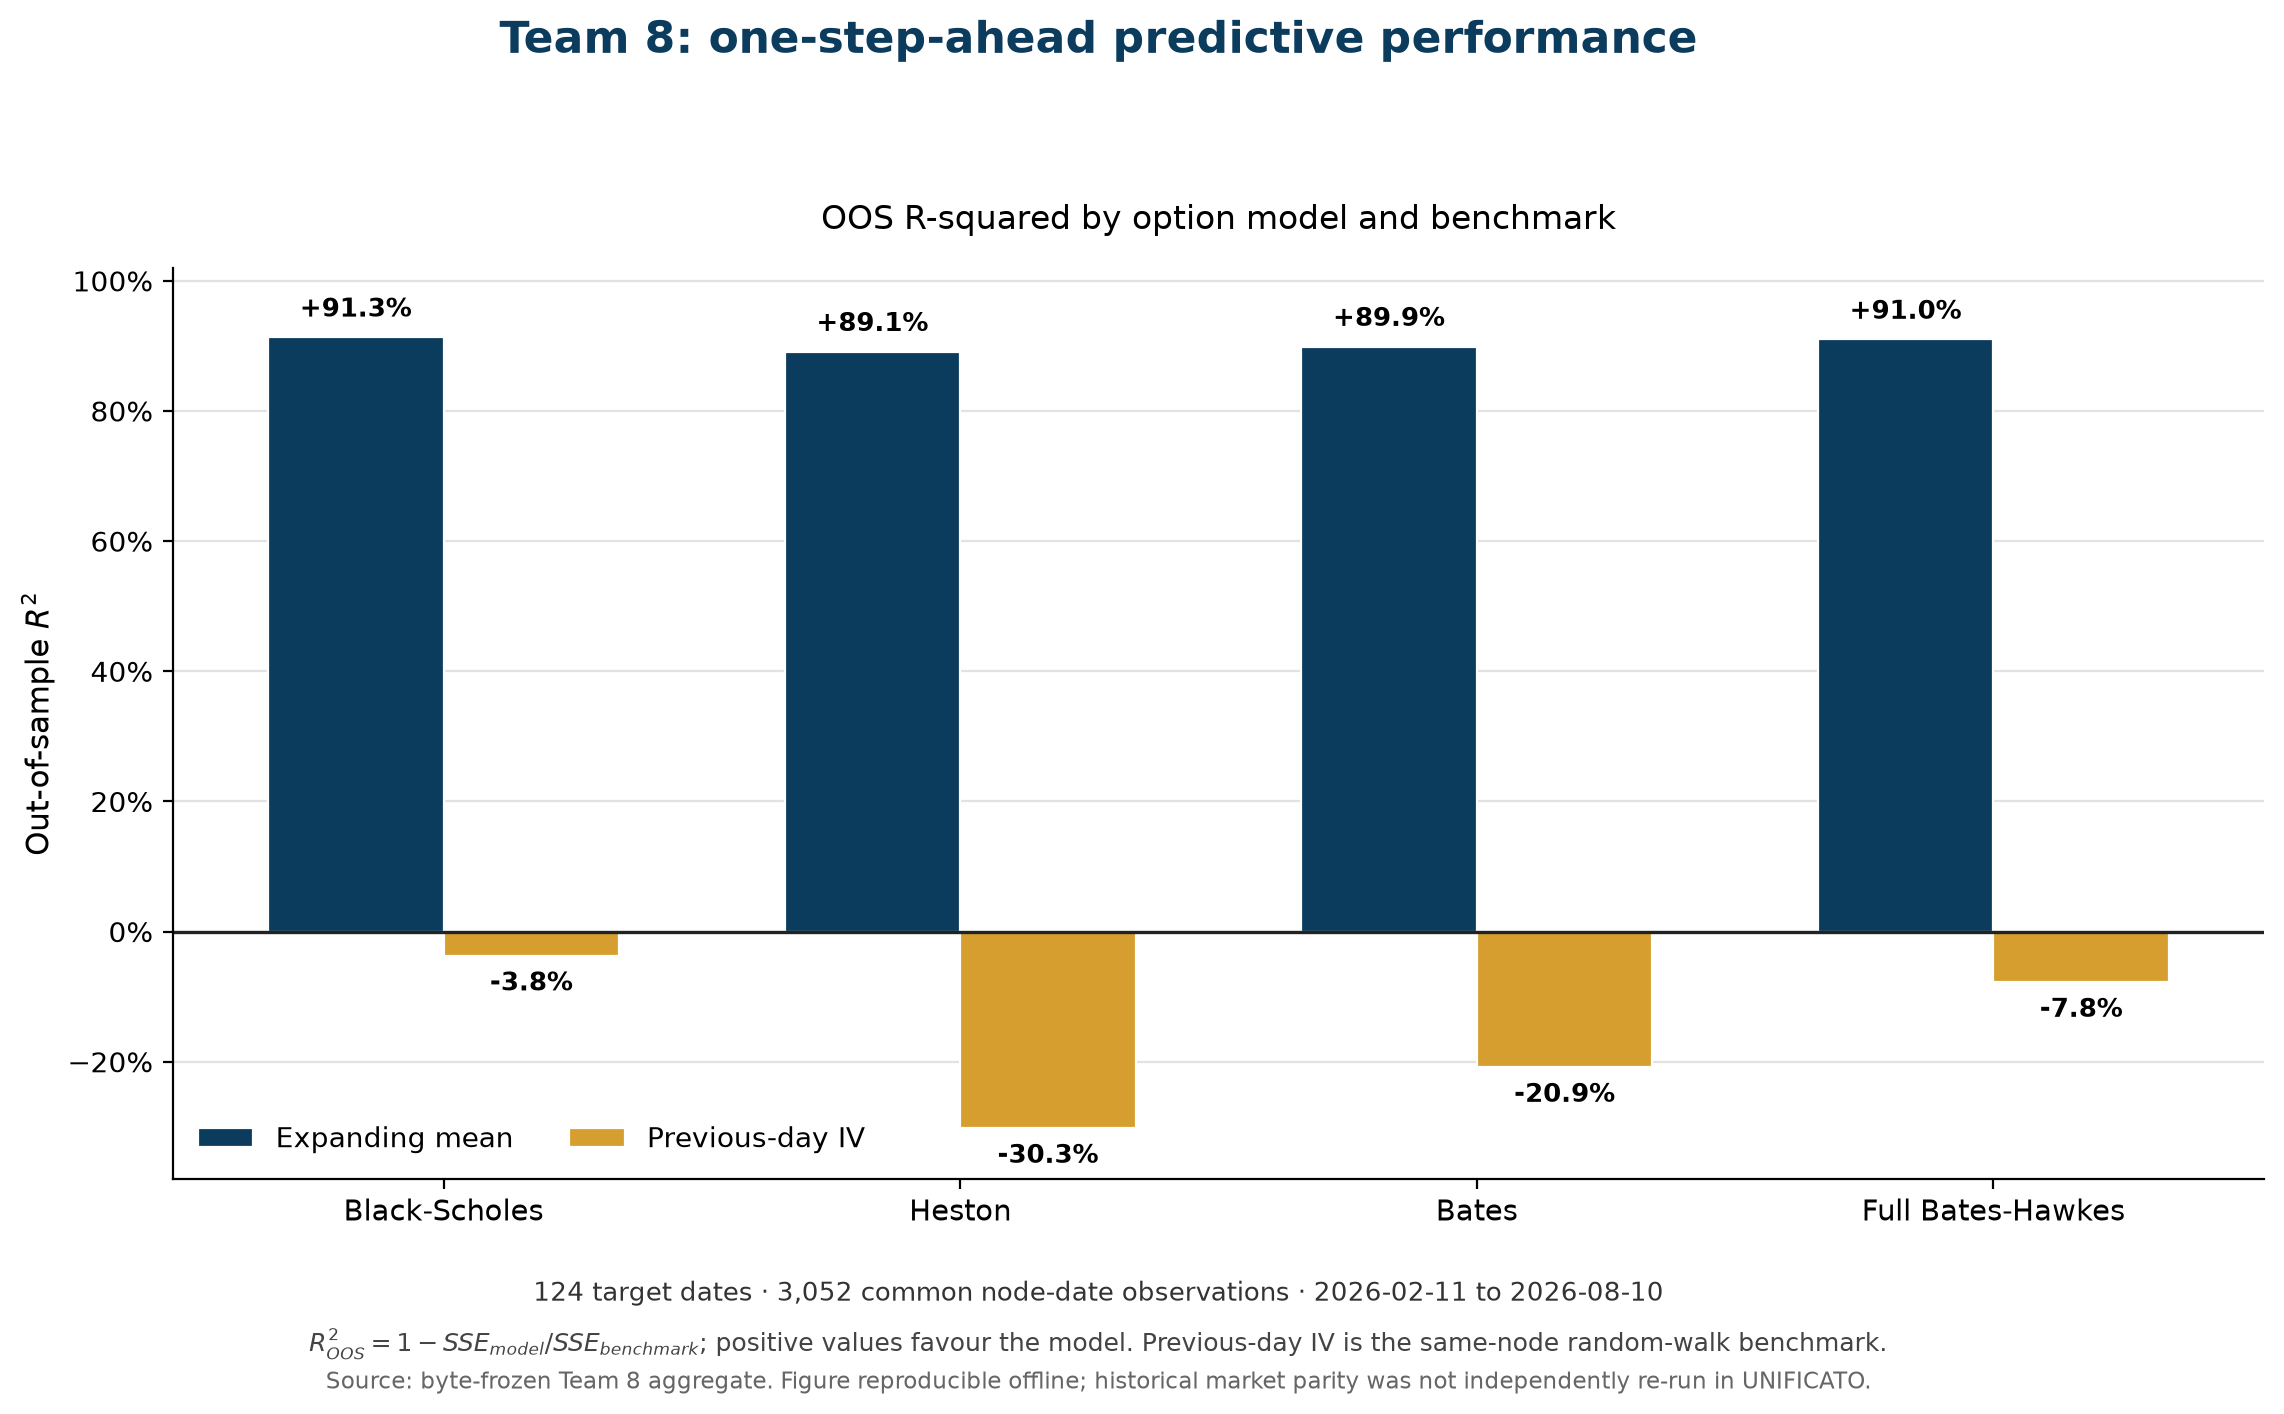
\includegraphics[width=0.95\columnwidth]{figures/online_oos_r2_by_benchmark.png}
  \captionof{figure}{One-step-ahead out-of-sample $R^2$. All four models improve on the expanding mean but fail to beat the previous-day IV surface. The test covers 124 target dates and 3,052 common node-date observations.}
  \label{fig:oos_r2}
\par}

\subsection{Predictive interpretation}
The OOS evidence prevents the in-sample ranking from being read as predictive dominance. Relative to an expanding mean, the four models explain a large share of one-step-ahead variation. Against the stronger same-node previous-day IV benchmark, every $R^2_{OOS}$ is negative; Black--Scholes also posts a slightly lower pooled RMSE than Full Bates--Hawkes. Structural flexibility therefore improves current-surface fit more clearly than short-horizon forecasting.

\begin{findingbox}[Model-risk conclusion]
Full Bates--Hawkes is primary for structural richness and current-surface calibration quality, but the valuation conclusion is reported across all four engines because the OOS evidence does not identify a dominant forecasting model.
\end{findingbox}

\subsection{Interpretive limitations}
The economic reading remains conditional: calibration is under $\mathbb Q$ without a validated $\mathbb Q\rightarrow\mathbb P$ map; GLD distributional shape is transferred without a one-for-one conversion to physical gold; market inputs are asynchronous; and the FCFF/equity bridge is not fully filing-reconciled. Debt, cash, minorities, non-operating assets and related bridge adjustments remain unresolved rather than silently inferred. The distributions are therefore research sensitivities, not fair values, confidence intervals or price targets.

{\centering
  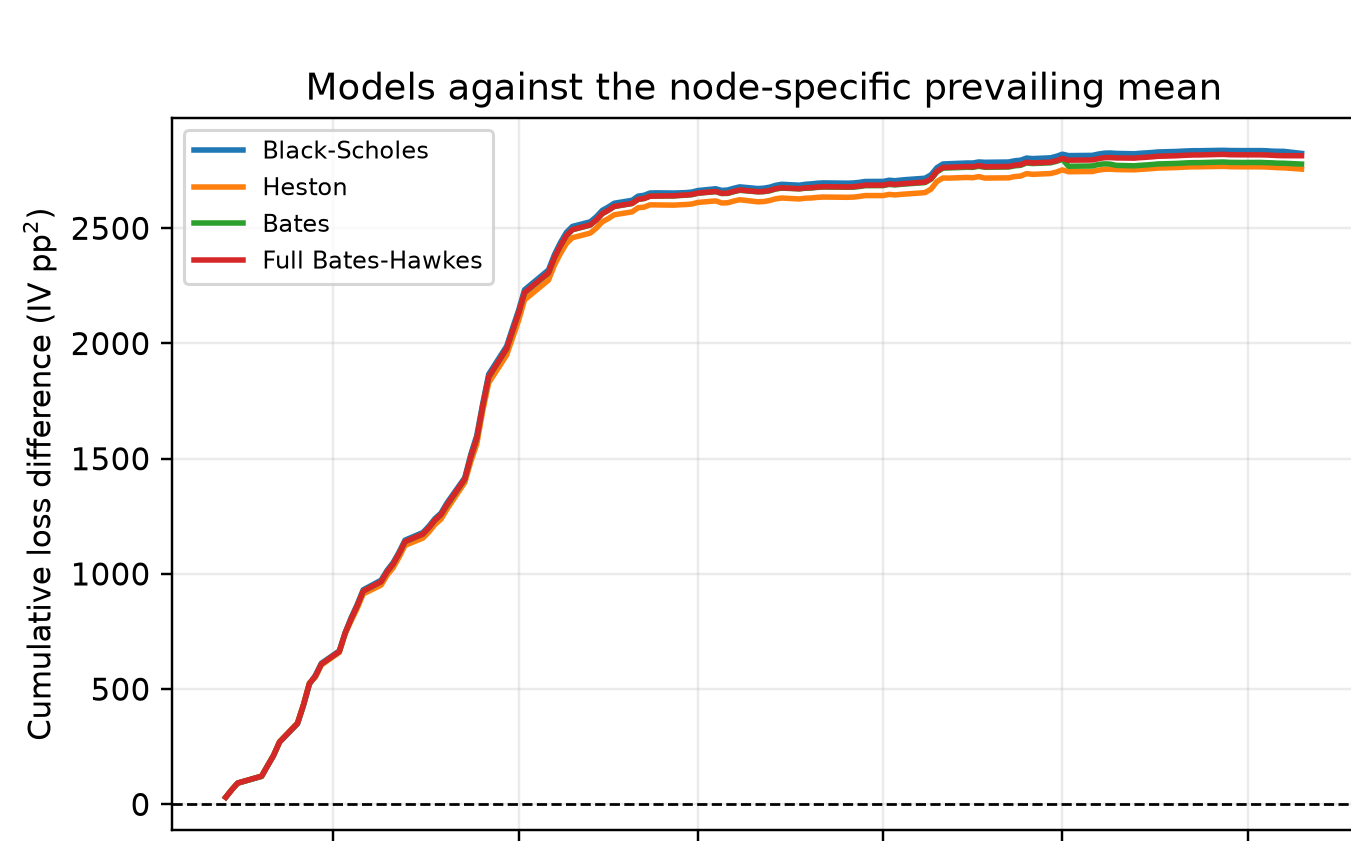
\includegraphics[width=0.95\columnwidth]{figures/welch_goyal_vs_mean.png}
  \captionof{figure}{Rolling Welch--Goyal cumulative loss difference against the node-specific prevailing mean. Upward movement favours the named model; all four specifications dominate this benchmark.}
  \label{fig:welch_goyal}
\par}


{\centering
  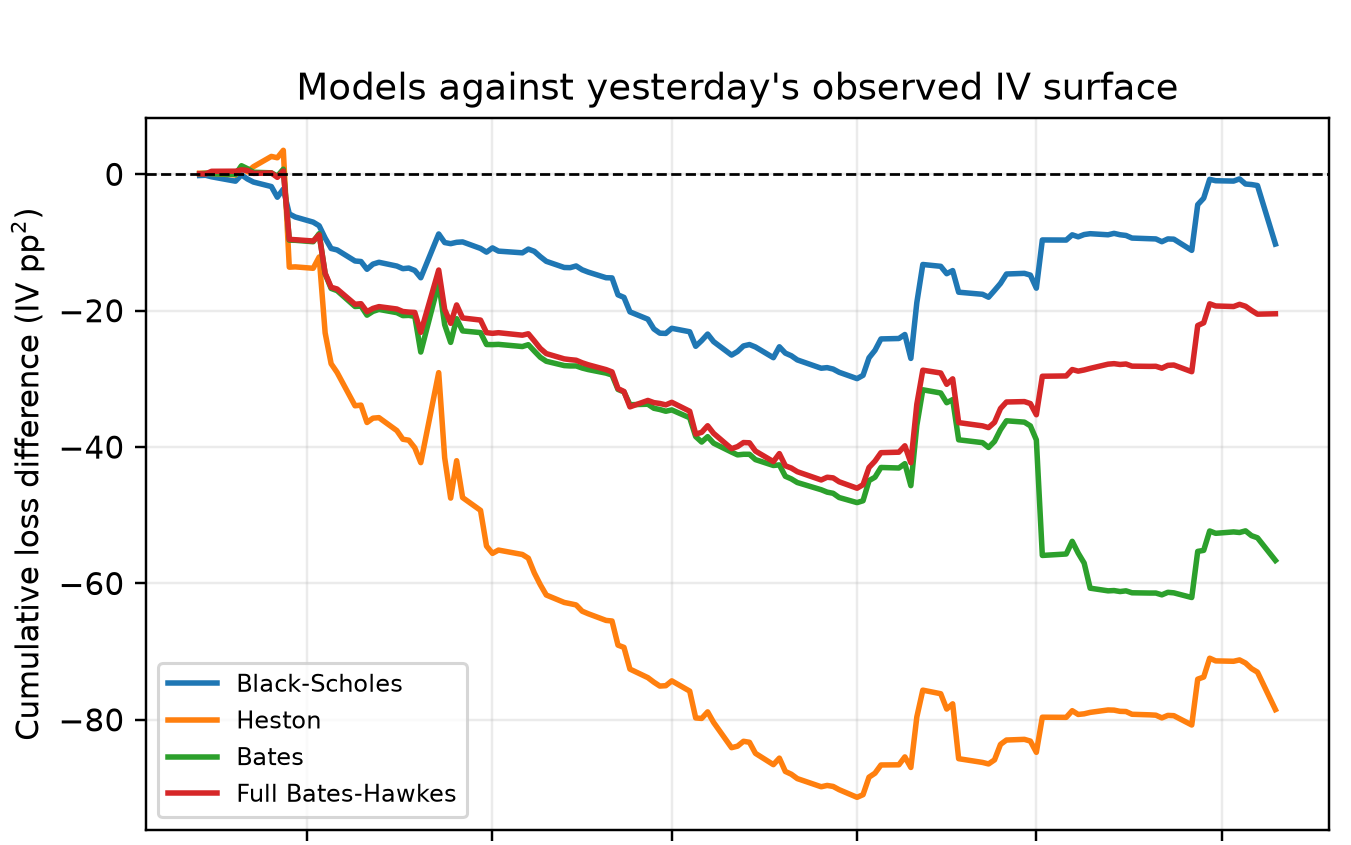
\includegraphics[width=0.95\columnwidth]{figures/welch_goyal_vs_previous_iv.png}
  \captionof*{figure}{\textbf{Figure~\ref{fig:welch_goyal} (continued).} Cumulative loss difference against the previous-day observed IV surface. Negative paths show that this stronger short-horizon benchmark remains superior.}
\par}

{\centering
  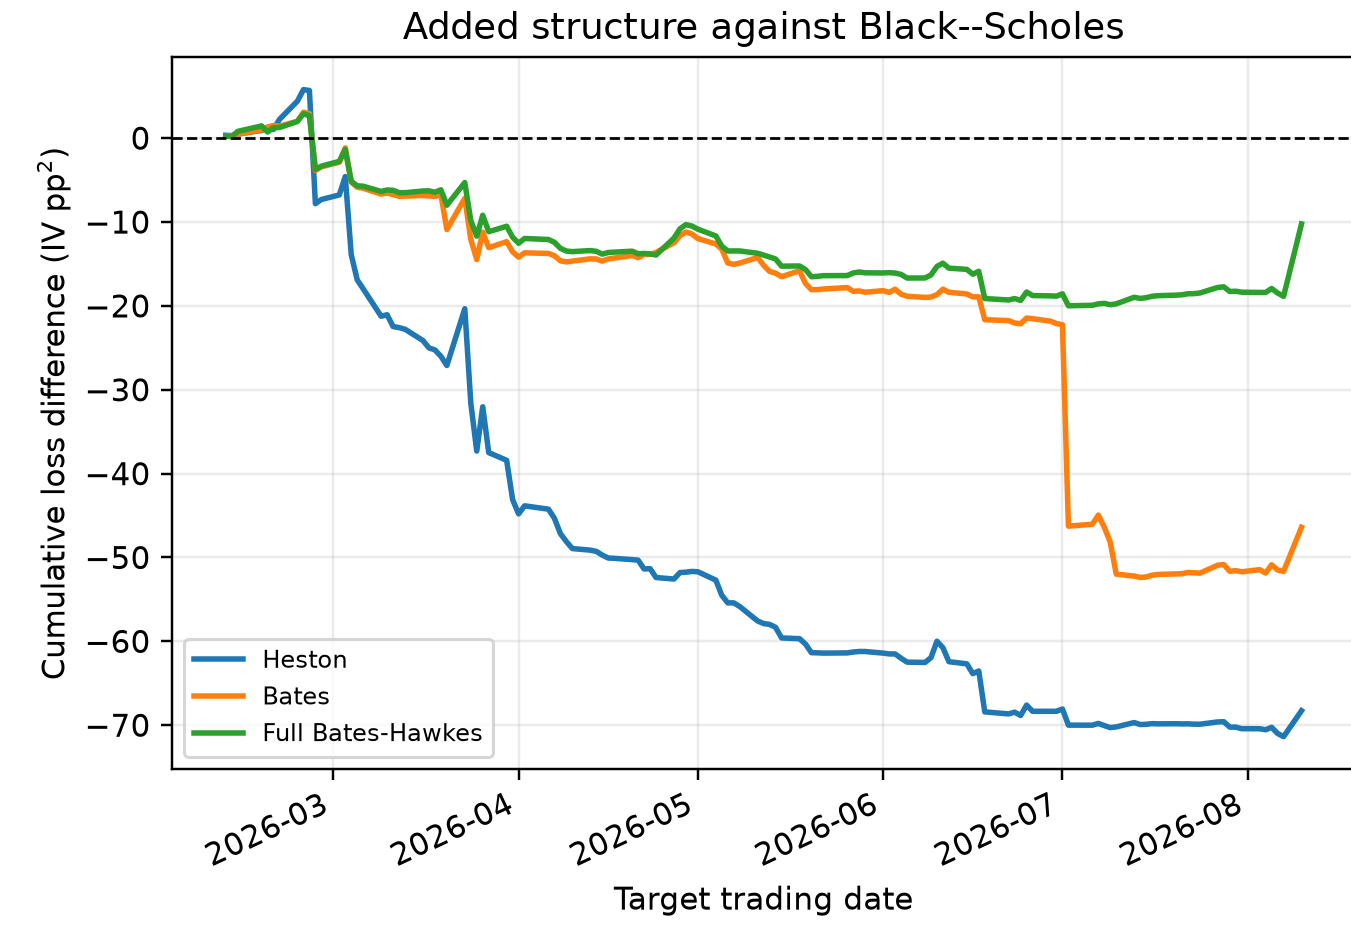
\includegraphics[width=0.95\columnwidth]{figures/welch_goyal_added_structure.png}
  \captionof*{figure}{\textbf{Figure~\ref{fig:welch_goyal} (continued).} Added stochastic-volatility and jump structure relative to Black--Scholes. Negative paths indicate that the simpler benchmark retains lower cumulative loss over this test.}
\par}

{\centering
  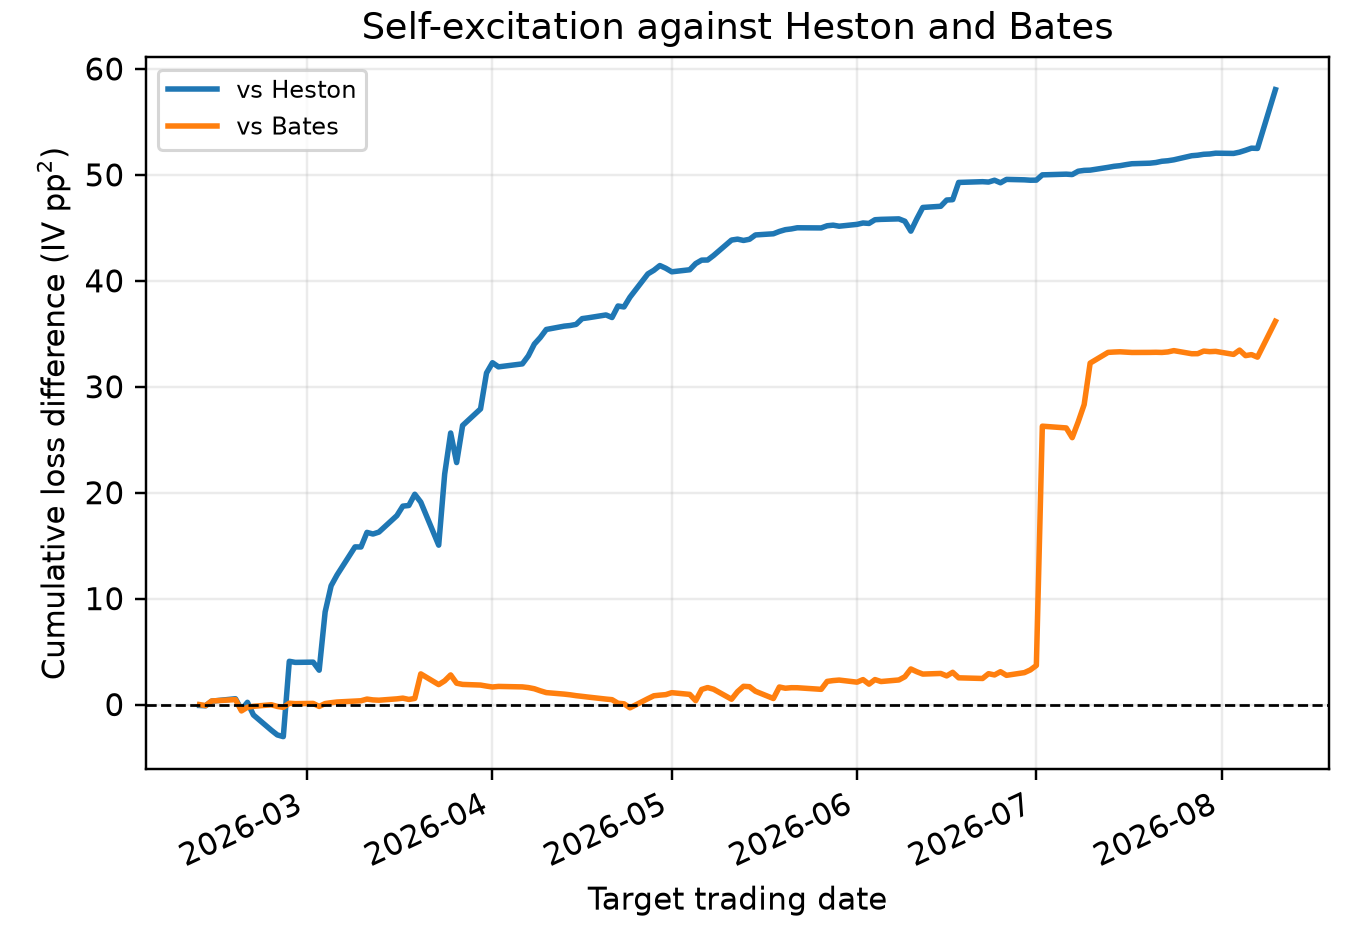
\includegraphics[width=0.95\columnwidth]{figures/welch_goyal_self_excitation.png}
  \captionof*{figure}{\textbf{Figure~\ref{fig:welch_goyal} (continued).} Full Bates--Hawkes relative to Heston and Bates. Positive paths favour the self-exciting specification within this pairwise comparison.}
\par}

\subsection{Jump-layer interpretation}
The self-exciting extension is motivated by clustered option-implied jump activity. Relative to the constant Poisson baseline, the Hawkes specification permits bursts of intensity followed by endogenous decay. In the current calibration the branching ratio is 0.02, so this channel is present but economically mild.

{\centering
  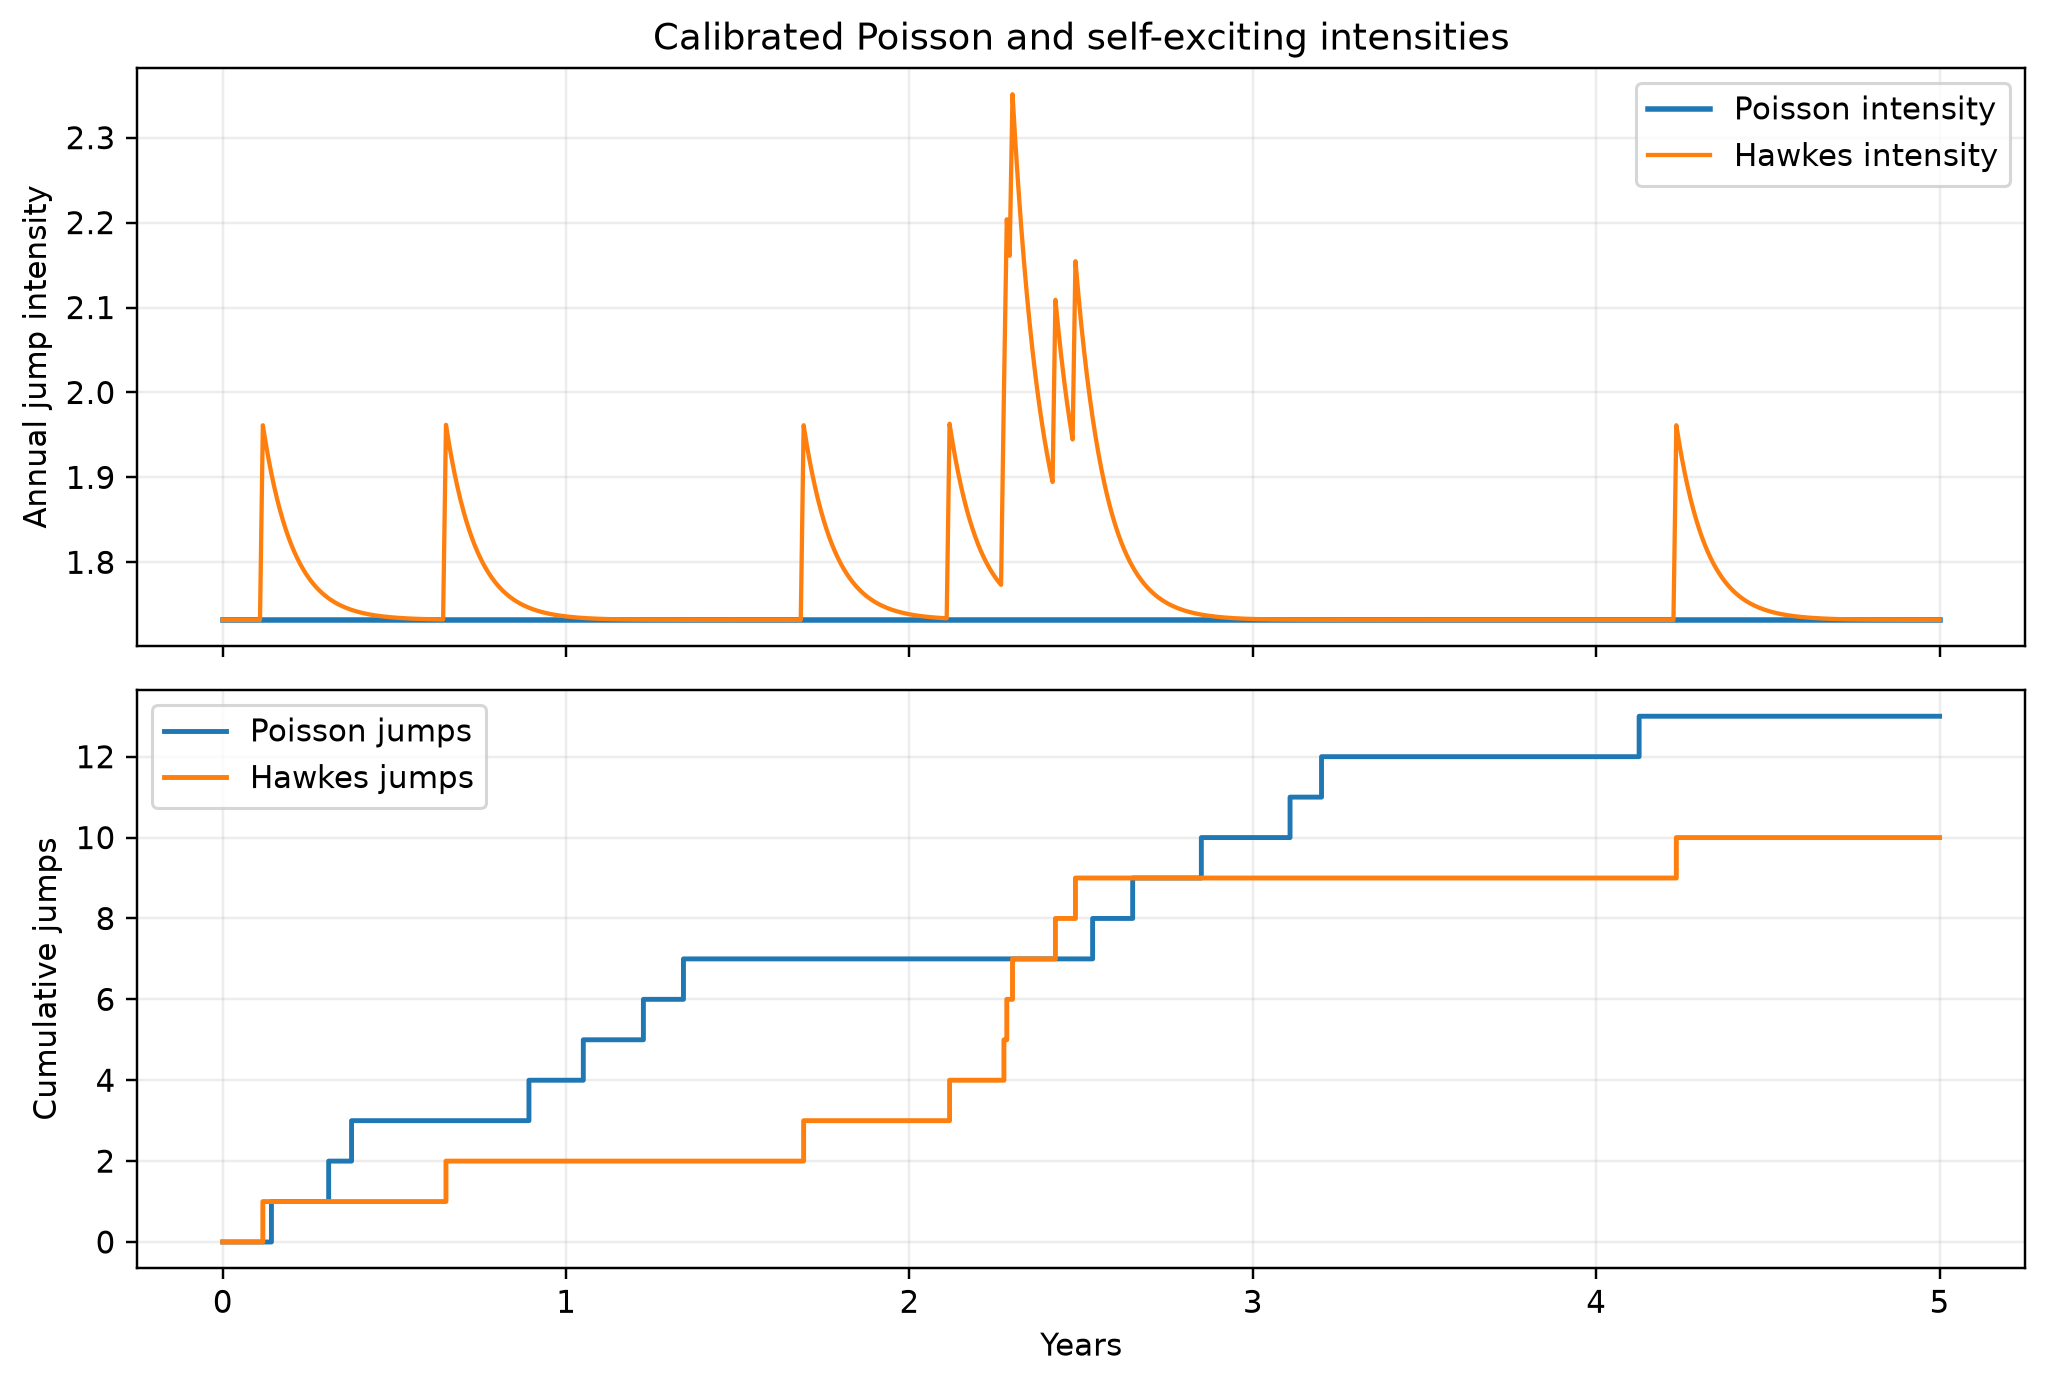
\includegraphics[width=0.95\columnwidth]{figures/hawkes_intensity_comparison.png}
  \captionof{figure}{Current Poisson and Hawkes intensity comparison. Hawkes allows clustered arrivals and decay, but the low fitted branching ratio keeps it close to the constant-intensity benchmark in this snapshot.}
  \label{fig:intensity_compare}
\par}

\section{Conclusion}

The experiment isolates the effect of stochastic gold dynamics while holding operations and corporate assumptions fixed. Under the refreshed 2 September inputs, all four conditional medians lie between USD~35.14 and USD~35.87, while the completed USD~44.13 market close remains above each median. This is a directional comparison, not a claim of market mispricing.

Model quality is multidimensional. Heston provides the strongest current-surface fit, whereas Full Bates--Hawkes produces the lowest date-equal rolling OOS loss. Its 0.5569 branching ratio is stationary but no longer economically negligible. None of the four models beats the interpolated persistence surface, although Full Bates--Hawkes comes closest. Team 4's updated operating layer uses Q1--Q2 2026 actuals and a separate Q3-onward forecast, but its uncertainty is frozen before model comparison.

The paper should therefore be read as a controlled attribution exercise. The explicit growth, WACC and terminal-value assumptions make the DCF auditable, but the terminal block still contributes about 78\% of positive enterprise value. Any fair-value interpretation would additionally require a reconciled commodity basis, physical-measure mapping, operating uncertainty and equity bridge.

\begin{findingbox}[Decision-relevant takeaway]
Under a common operating and DCF contract, changing the stochastic gold engine can affect both the central valuation signal and tail risk. The current architecture is informative for model comparison, but it is not yet a filing-reconciled fair-value model.
\end{findingbox}


\begingroup
\setlength{\bibsep}{0.6pt}
\fontsize{6.75}{7.75}\selectfont
\input{main.bbl}
\endgroup

\end{multicols}

\end{document}
